\documentclass[11pt,a4paper]{report}
\usepackage[utf8]{inputenc}
\usepackage[spanish]{babel}
\usepackage{graphicx}
\usepackage{makeidx}
\usepackage[pdftex,
			pagebackref=true,
            colorlinks=true,
            linkcolor=blue!70!black,
            urlcolor=blue!70!black,
            citecolor=blue!70!black,
            unicode
			]{hyperref}
\usepackage[margin=3cm]{geometry}
\usepackage{makeidx}
\usepackage{multicol}
\usepackage{multirow}
\usepackage[nottoc]{tocbibind}
\usepackage{longtable}
\usepackage[x11names,table]{xcolor}
\usepackage{amsmath,amssymb,amsfonts,latexsym,cancel}
\usepackage{amsthm}
\usepackage{color}
\usepackage{algorithmic}
\usepackage[chapter]{algorithm}
\usepackage{listings}
\usepackage{caption}
\usepackage{subcaption}
\usepackage{float}
\usepackage{forloop}
\usepackage{tikz}
\usepackage{xstring}
\usepackage{fancyhdr}
\usepackage{lipsum}

\pagestyle{fancy}
\lhead{\slshape\nouppercase{\rightmark}}
\rhead{\thepage}

%\renewcommand{\thesubfigure}{\arabic{subfigure}}

\lstset{ %
  xleftmargin=40pt,
  backgroundcolor=\color{white},   % choose the background color; you must add \usepackage{color} or \usepackage{xcolor}
  basicstyle=\footnotesize,        % the size of the fonts that are used for the code
  breakatwhitespace=false,         % sets if automatic breaks should only happen at whitespace
  breaklines=true,                 % sets automatic line breaking
  captionpos=b,                    % sets the caption-position to bottom
  commentstyle=\color{green},    % comment style
  deletekeywords={...},            % if you want to delete keywords from the given language
  escapeinside={\%*}{*)},          % if you want to add LaTeX within your code
  extendedchars=true,              % lets you use non-ASCII characters; for 8-bits encodings only, does not work with UTF-8
  frame=none,                    % adds a frame around the code
  keepspaces=true,                 % keeps spaces in text, useful for keeping indentation of code (possibly needs columns=flexible)
  keywordstyle=\color{blue},       % keyword style
  language=C++,                 % the language of the code
  morekeywords={*,...},            % if you want to add more keywords to the set
  numbers=left,                    % where to put the line-numbers; possible values are (none, left, right)
  numbersep=10pt,                   % how far the line-numbers are from the code
  numberstyle=\color{gray}, % the style that is used for the line-numbers
  rulecolor=\color{black},         % if not set, the frame-color may be changed on line-breaks within not-black text (e.g. comments (green here))
  showspaces=false,                % show spaces everywhere adding particular underscores; it overrides 'showstringspaces'
  showstringspaces=false,          % underline spaces within strings only
  showtabs=false,                  % show tabs within strings adding particular underscores
  stepnumber=1,                    % the step between two line-numbers. If it's 1, each line will be numbered
  stringstyle=\color{red},     % string literal style
  tabsize=4,                       % sets default tabsize to 2 spaces
  title=\lstname                   % show the filename of files included with \lstinputlisting; also try caption instead of title
}

\newtheoremstyle{custom}
{\topsep}   % Space above
{\topsep}   % Space below
{\slshape}  % Body font
{0pt}       % Indent amount (empty value is the same as 0pt)
{\bfseries} % Theorem head font
{}          % Punctuation after theorem head
{5pt plus 1pt minus 1pt} % Space after theorem head
{\thmname{#1}\thmnumber{ #2}\thmnote{ {\it #3}}\\} % Theorem head spec

\theoremstyle{custom}
\newtheorem{mydef}{Definición}
\numberwithin{mydef}{chapter}

\addto\captionsspanish{
\renewcommand{\abstractname}{Resumen}
\renewcommand{\tablename}{\bf Tabla}
\renewcommand{\partname}{Parte}
\renewcommand{\appendixname}{Anexo}
\renewcommand{\figurename}{\bf Figura}
\renewcommand{\chaptername}{Capítulo}
\renewcommand{\contentsname}{Índice}
\renewcommand{\listtablename}{Lista de Tablas}
\renewcommand{\listfigurename}{Lista de Figuras}
\renewcommand{\bibname}{Bibliografía}
\floatname{algorithm}{Algoritmo}
\renewcommand{\algorithmicrequire}{\textbf{Entrada:}}
\renewcommand{\algorithmicensure}{\textbf{Salida:}}
}

\def\myauthor{Santiago Javier Vilca Limachi}
\def\mytitle{Aplicación de modelos de Deep Learning para la detección de señales sísmicas P y S en sismogramas.}

\title
{
	
\includegraphics[width=0.32\textwidth]{figures/unsa}\\\vspace{0.5cm}
	\large UNIVERSIDAD NACIONAL DE SAN AGUSTÍN\\ 
	\sc Facultad de Ingeniería de Producción y Servicios\\ 
	Escuela Profesional de Ciencia de la Computación\\\vspace{3cm}
	\Large\bf\mytitle\\\vspace{1.5cm}
}

\author{Tesis presentada por:\\{\Large\sc\myauthor}\\\\
		Para optar el Título Profesional de\\Licenciado en Ciencia de la Computación.}

\date{\vspace{3cm}\sc Arequipa\\2017}


\def\figura#1#2#3
{
\begin{figure}[!h]
\centering\includegraphics[width = #2\textwidth]{figures/#1}
\caption{\em #3}\label{#1}
\end{figure}
}

% size, figures array, label, caption
\def\images#1#2#3#4
{
	\begin{figure}[!htb]
		\centering
		\foreach \imagepath/\imagename/\imagecaption in #2
		{
			\subcaptionbox{\label{\imagepath/\imagename} \em \imagecaption}
			{\includegraphics[width=#1\textwidth]{\imagepath/\imagename}}
		}
		\caption{\em #4}\label{#3}
	\end{figure}
}

\def\myimage#1#2%
{%
	\begin{figure}[!htb]
		\centering
		\input{#1}
		\caption{\em #2}\label{#1}
	\end{figure}
}

\newcommand{\tabla}[3]
{
\begin{table}[!h]
\centering#3
\caption{\em #2}\label{#1}
\end{table}
}

\def\refcap#1{\hyperref[#1]{Capítulo \ref{#1}}}
\def\refsec#1{\hyperref[#1]{Sección \ref{#1}}}
\def\reffig#1{\hyperref[#1]{Figura \ref{#1}}}
\def\reftab#1{\hyperref[#1]{Tabla \ref{#1}}}

%%%%%%%%%%%%%%%%%%%%%%%%%%%%%%%%%%%%%%%%%%%%%%%%%%%%%%%%%%%%%%%%%%%%%%%%%%%%%%%%%%%%%%%%%%%%%%%%%%%%%%%%%%%%%%%%%%%%%%%%%%%%%%%%%%

\begin{document}

\maketitle

\begin{titlepage}
\begin{center}
{\Large\sc\myauthor}\\\vspace{2cm}
{\Large\mytitle}\\\vspace{3cm}
\end{center}
\null\hfill
\begin{minipage}{0.48\textwidth}
\large
Tesis presentada para optar el Título Profesional de
Licenciado en Ciencia de la Computación.
\end{minipage}

\bigskip\vspace{2cm}
\large Aprobada en Mayo del 2025.\\\vspace{2cm}

\null\hfill
\begin{minipage}{0.52\textwidth}
\large
\begin{itemize}
\item[] \textbf{Miembros del Jurado:}
\item[\bf Asesor:] Prof.\ Cristian José López Del Álamo
\item[\bf Presidente:] Prof.\ Wilber Ramos Lovón
\item[\bf Secretario:] Prof.\ Juan Carlos Gutiérrez Cáceres
\end{itemize}
\end{minipage}

\bigskip\vspace{4cm}
\begin{center}
\large\sc Arequipa\\2017
\end{center}
\end{titlepage}

\begin{titlepage}
\null\vfill\null\hfill\em Este trabajo está dedicado a mis padres.
\end{titlepage}

\setlength{\parskip}{1em}
\begin{abstract}

La detección temprana y precisa de las fases sísmicas P y S en registros sismológicos es una tarea crítica en la implementación de sistemas de alerta temprana ante terremotos (EEWS). La identificación manual de estas fases es laboriosa, propensa a errores y difícil de escalar, especialmente en regiones con alta actividad sísmica y baja densidad de estaciones. En este contexto, los modelos basados en aprendizaje profundo han demostrado ser una alternativa prometedora para automatizar esta tarea, destacando entre ellos el modelo \textit{EQTransformer}, una arquitectura basada en redes neuronales recurrentes y convolucionales con mecanismos de atención.

La presente tesis propone una mejora al modelo \textit{EQTransformer} mediante la incorporación de una capa de multiatención jerárquica basada en \textit{Swin Transformer}, una arquitectura reciente y eficiente que permite capturar relaciones espaciales y temporales a múltiples escalas dentro de secuencias de datos. Esta modificación tiene como objetivo aumentar la capacidad del modelo para detectar patrones complejos en señales sísmicas, especialmente en escenarios de bajo nivel de señal o presencia de ruido.

Se construyó un \textit{pipeline} completo de procesamiento, que incluye adquisición y preprocesamiento de señales, entrenamiento del modelo, identificación de fases sísmicas y evaluación de parámetros de evento. La arquitectura propuesta fue entrenada utilizando un conjunto de datos sísmicos reales, etiquetados con fases P y S, y fue validada con métricas estándar como precisión, sensibilidad y \textit{F1-score}. Además, se emplearon técnicas de interpretabilidad para analizar las regiones de la señal más relevantes para la predicción del modelo.

Los resultados muestran que la incorporación del bloque \textit{Swin Transformer} mejora significativamente el rendimiento del modelo en comparación con la versión original de \textit{EQTransformer}, especialmente en señales ruidosas o con fases sísmicas poco claras. Asimismo, el modelo modificado mostró mayor robustez en generalización, lo cual es crucial para su aplicación en tiempo real en distintas regiones geográficas.

Este trabajo contribuye al campo de la sismología computacional al ofrecer un enfoque más potente y flexible para la detección automática de fases sísmicas, y sienta las bases para futuras investigaciones en sistemas inteligentes de alerta temprana impulsados por modelos jerárquicos de atención.

\end{abstract}

%\chapter*{Agradecimiento}

\lipsum


\setlength{\parskip}{0em}
\tableofcontents
\listoffigures
\listoftables

\setlength{\parskip}{1em}
% Introduction and Background
\chapter{Introducción}\label{introduction}

Los terremotos representan uno de los fenómenos naturales más devastadores, con un impacto significativo en la vida humana, las infraestructuras y las economías globales. Un terremoto se produce debido al movimiento súbito de las placas tectónicas de la Tierra, liberando una enorme cantidad de energía en forma de ondas sísmicas. Estas ondas pueden causar una destrucción masiva y pérdidas humanas, por lo que la detección temprana y precisa de terremotos es de vital importancia para mitigar sus efectos destructivos \cite{Joswig} \cite{havskov2008processing}.

Las ondas sísmicas generadas por un terremoto se dividen principalmente en dos tipos: las ondas P (primarias) y las ondas S (secundarias). Las ondas P son las primeras en llegar a las estaciones sísmicas debido a su mayor velocidad, mientras que las ondas S, aunque más lentas, son generalmente más destructivas. El reconocimiento preciso de estas fases es crucial, ya que permite determinar la localización y magnitud del terremoto, facilitando una respuesta rápida y efectiva ante emergencias \cite{havskov2008processing}.

El problema de reconocer y detectar las fases P y S de manera automática y precisa es un desafío significativo en sismología. La identificación manual de estas fases es laboriosa y propensa a errores, especialmente en datos ruidosos o complejos. Aquí es donde entra en juego la tecnología de redes neuronales profundas, específicamente las redes transformer, que han demostrado una capacidad notable para manejar secuencias de datos y detectar patrones complejos \cite{havskov2008processing} \cite{SUGONDO2021e08605}.

En sismología, las ondas P y S son fundamentales para entender la propagación de energía sísmica a través de la Tierra. Las ondas P, también conocidas como ondas primarias o longitudinales, se propagan a través de sólidos, líquidos y gases y se describen por la ecuación de onda para ondas longitudinales \cite{chapman2004fundamentals} .
\begin{equation*}
\frac{\partial^{2}u}{\partial t^{2}} = c_{p}^{2}\nabla^{2}u
\end{equation*}

Donde $u$ es la función de desplazamiento, $t$ es el tiempo, y $c_{P}$ es la velocidad de la onda P, determinada por las propiedades elásticas del medio. Por otro lado, las ondas S, o secundarias, se mueven solo a través de medios sólidos y su movimiento se rige por la ecuación \cite{chapman2004fundamentals}.
\begin{equation*}
\frac{\partial^{2}u}{\partial t^{2}} = c_{s}^{2}\nabla^{2}u
\end{equation*}

Donde $c_{S}$ es la velocidad de la onda S, relacionada con la velocidad de propagación del sonido $v_{s}$. Estas ondas causan movimientos perpendiculares a la dirección de propagación y no pueden atravesar medios líquidos o gaseosos debido a su naturaleza de corte. Comprender estas características es esencial para la evaluación precisa de eventos sísmicos y para mejorar las estrategias de mitigación de riesgos asociados a terremotos \cite{chapman2004fundamentals}.

Este artículo presenta una propuesta para el reconocimiento y la detección de fases sísmicas P y S utilizando un modelo transformer de multiatención. Los objetivos de este estudio son: Mostrar un modelo transformer eficiente para la detección automática de las fases P y S. Y Evaluar el rendimiento del modelo en comparación con métodos tradicionales y otros enfoques basados en aprendizaje profundo.

La estructura del artículo se organiza de la siguiente manera: en primer lugar, se presentan los trabajos relacionados, donde se revisan los estudios previos y los métodos existentes para la detección de fases sísmicas. En segundo lugar, se expone la propuesta, que incluye una descripción detallada de la arquitectura del modelo basado en transformers, los parámetros utilizados y la configuración del modelo, así como una presentación del conjunto de datos empleado para el entrenamiento y evaluación. En tercer lugar, se discuten los resultados obtenidos, especificando el entorno de hardware y software utilizado para los experimentos, las curvas de aprendizaje observadas durante el entrenamiento, los procedimientos de prueba y validación, y los resultados cuantitativos en términos de precisión y eficiencia. Finalmente, se incluye una tabla comparativa donde se evalúa el rendimiento del modelo propuesto frente a otros enfoques existentes.

\section{Contexto}

Los terremotos son desastres naturales extremadamente destructivos e impredecibles que crean una gran amenaza para la vida e infraestructura humana. En las últimas décadas, varios terremotos importantes han causado una gran cantidad de víctimas mortales y heridas generalizadas. Por ejemplo, el terremoto de Haití -Aarth en 2010, con un momento (MW) 7.0, alrededor de 300,000 muertes, causó 1,5 millones de personas sin hogar. Del mismo modo, el Tohokus fue causado por un terremoto en Japón 2011 con un MW de 9.1 aproximadamente 15,641 muertes y lesiones a un valor de 211 mil millones, que se convirtió en el desastre natural más caro de la historia. Estos eventos enfatizan la necesidad crítica de una detección efectiva y rápida de terremotos y sistemas de reacción.

Los primeros sistemas de alarma de terremotos (EEWS) están diseñados para detectar las primeras ondas P, menos destructivas, terremotos y proporcionar advertencias antes de que lleguen las ondas W más destructivas. El desarrollo de estos sistemas ha sido una herramienta importante para reducir la influencia de los terremotos, permitiendo a las personas tomar medidas preventivas y permitir que sistemas automatizados como trenes y maquinaria industrial eviten daños importantes.

Países como Japón, México y Estados Unidos han introducido un complejo EEW que envía alarmas de la sociedad a los ciudadanos en regiones sísmicamente activas. Por ejemplo, el EEWS japonés ha sido esencial para reducir los efectos de los terremotos a través de alarmas a través de teléfonos móviles, televisión y radio. Del mismo modo, el sistema de alarma sísmica mexicana (SASMEX) advirtió al público desde 1993, lo que redujo significativamente a las víctimas en las zonas urbanas. Sin embargo, la eficiencia de la densidad y el recubrimiento de estas redes sísmicas, así como la precisión y velocidad de los algoritmos subyacentes, depende de los datos sísmicos.

El método tradicional de detección de terremotos depende en gran medida de los sismómetros y las redes algorítmicas, como el método promedio temporal / a largo plazo (ST / LTA) utilizado para determinar la actividad sísmica, identificando un aumento repentino en la amplitud de la señal. Si bien estos métodos han sido exitosos, se enfrentan a una serie de restricciones, como las redes sísmicas distribuidas en algunas regiones que evitan los tiempos de detección, y los algoritmos, como STA/LTA, pueden tener dificultades en una marca baja en un determinado entorno que conduce a eventos positivos positivos falsos positivos o no abiertos. Estos problemas enfatizan la necesidad de la detección avanzada de tecnologías que proporcionan ansiedad más rápida y precisa. La inteligencia artificial (IA) se convierte en un instrumento transformador en sismología que ofrece nuevos métodos para determinar y caracterizar los eventos sísmicos. Los algoritmos de aprendizaje automático (ML) y aprendizaje profundo (DL) son particularmente adecuados para grandes conjuntos de datos, identificación y decisiones rápidas sin requerir una amplia gama de intervención manual. Estos métodos ya se han utilizado en diversas áreas, como la salud y la astrofísica, y su potencial en la sismología se está volviendo cada vez más obvio.


% \lipsum 
% \figura{csunsa}{0.6}{CS UNSA\cite{FuentesPerez2017}}

\section{Contribuciones}

En este trabajo, proponemos un modelo transformer de multiatención para el reconocimiento y detección de fases sísmicas P y S. El modelo aprovecha la capacidad de los transformers para manejar secuencias de datos de manera efectiva, capturando dependencias a largo plazo y patrones complejos en las señales sísmicas.

La arquitectura de este modelo se basa en la estructura de multiatención del transformer, que permite al modelo enfocarse en diferentes partes de la señal de entrada de manera simultánea. Este enfoque es particularmente útil en la sismología, donde las características relevantes pueden estar dispersas a lo largo de la señal. Al aplicar múltiples cabezas de atención, el modelo puede extraer y combinar información de varias escalas temporales y frecuencias \cite{46201}, mejorando la precisión en la detección de las fases P y S.

El proceso de entrenamiento del modelo se lleva a cabo utilizando un conjunto de datos sísmicos etiquetados (este punto se explicara en la sub seccion dataset), donde se conocen las ubicaciones temporales de las fases P y S. Durante el entrenamiento, el modelo aprende a identificar patrones característicos de estas fases y a distinguirlas de otros tipos de ruido y señales sísmicas. Una vez entrenado, el modelo puede aplicarse en tiempo real para el monitoreo sísmico, proporcionando una herramienta robusta para la detección automática de eventos sísmicos.

El pipeline del sistema propuesto consta de varias etapas fundamentales, cada una de las cuales puede abordarse con distintos enfoques dentro del ámbito del aprendizaje automático y procesamiento de señales. Estas etapas incluyen:

\begin{itemize}
\item \textbf{Adquisición de datos}: En esta fase se recogen las señales sísmicas crudas provenientes de sensores locales, los cuales pueden ser de diferentes tipos (geófonos, acelerómetros, etc.). Se prevé utilizar estaciones tanto reales como simuladas para entrenar y validar el modelo.

\item \textbf{Preprocesamiento}: Incluye técnicas como normalización, filtrado por bandas de frecuencia y segmentación de ventanas de tiempo. Esta etapa también contempla la identificación de ruido para mejorar la relación señal-ruido (SNR) en las entradas al modelo.

\item \textbf{Detección de eventos}: En esta etapa se plantea el uso de modelos de aprendizaje profundo, particularmente arquitecturas basadas en Swin Transformers jerárquicos, aunque también se consideran modelos como EQTransformer, ICAT-net o variantes livianas optimizadas de Transformers.

\item \textbf{Identificación de fases sísmicas (picking de fases P y S)}: Esta subetapa puede implementarse mediante el mismo modelo de detección o como una etapa independiente, dependiendo del rendimiento observado. Técnicas como mecanismos de atención espacial y temporal pueden ser aplicadas para mejorar la precisión de los tiempos de arribo.

\item \textbf{Estimación de parámetros de la fuente}: Incluye el cálculo de magnitud, distancia epicentral, back-azimuth y profundidad hipocentral. Esta etapa podría beneficiarse de modelos adicionales entrenados específicamente para regresión multivariada, posiblemente con arquitecturas tipo Transformer o modelos híbridos \ref{Fig:Pipeline}.

\item \textbf{Interpretabilidad del modelo}: Se explorarán técnicas como SHAP (SHapley Additive exPlanations), Grad-CAM adaptado a series temporales o atención visualizable para analizar qué aspectos de la señal influyen más en la detección y caracterización del evento, con el objetivo de extraer conocimiento físico útil a partir del modelo \ref{Fig:Pipeline}.

\item \textbf{Generación de alerta}: Finalmente, el sistema debe emitir una alerta local en caso de detectarse un sismo significativo, en base a umbrales configurables. Esta alerta puede ser utilizada para activar sistemas automáticos o notificar a usuarios por medios definidos \ref{Fig:Pipeline}.
\end{itemize}

\begin{figure*}[htbp]
\begin{center}
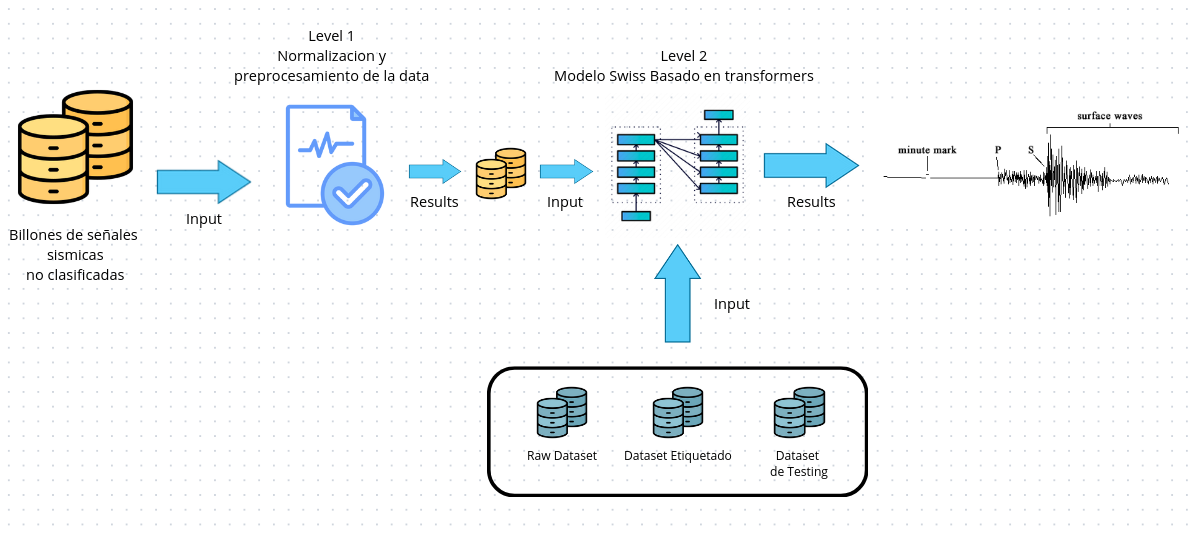
\includegraphics[scale=0.4]{figures/PIPELINE.png}
\caption{Pipeline del modelo propuesto.}
\label{Fig:Pipeline}
\end{center}
\end{figure*}

\section{Estructura de la tesis}

La presente tesis se encuentra organizada en cinco capítulos, los cuales se detallan a continuación:

\begin{itemize}
    \item \textbf{Capítulo 1 – Introducción}: Se presenta el contexto general del problema, así como la importancia de la detección temprana de ondas sísmicas. Se describe el objetivo principal del trabajo, la motivación detrás del uso de modelos basados en \textit{deep learning}, especialmente \textit{transformers}, y las contribuciones específicas de la investigación. Finalmente, se detalla la organización general del documento.

    \item \textbf{Capítulo 2 – Estado del Arte}: Se realiza una revisión de los métodos existentes para la detección de fases sísmicas, tanto tradicionales como basados en técnicas de inteligencia artificial. Se discuten modelos relevantes como \textit{EQTransformer}, \textit{PhaseNet}, y otras arquitecturas de redes neuronales profundas, así como sus fortalezas, limitaciones y oportunidades de mejora.

    \item \textbf{Capítulo 3 – Metodología}: Se describe detalladamente el enfoque propuesto, incluyendo la arquitectura del modelo \textit{transformer}, las técnicas de preprocesamiento aplicadas a las señales sísmicas, y la configuración del proceso de entrenamiento. Además, se presenta el conjunto de datos utilizado, las métricas de evaluación y el \textit{pipeline} completo del sistema.

    \item \textbf{Capítulo 4 – Resultados y análisis}: Se presentan los resultados obtenidos por el modelo propuesto en distintas métricas de desempeño. Se comparan estos resultados con enfoques tradicionales y modelos existentes. También se analiza la interpretabilidad del modelo y su capacidad para generalizar a nuevos datos.

    \item \textbf{Capítulo 5 – Conclusiones y trabajos futuros}: Se resumen las principales conclusiones de la investigación, destacando los logros alcanzados y las limitaciones identificadas. Finalmente, se proponen líneas futuras de trabajo orientadas a mejorar el rendimiento del modelo, adaptarlo a otras regiones geográficas, y explorar nuevas aplicaciones dentro del ámbito de la sismología computacional.
\end{itemize}

\chapter{Estado del Arte}\label{background}

\section{Consideraciones Iniciales}

La detección precisa del tiempo de llegada de las fases sísmicas, especialmente la onda P (P-wave), constituye un componente crítico en múltiples aplicaciones dentro de la sismología, como la localización de eventos sísmicos, la estimación de magnitud, y la caracterización de la estructura del subsuelo. La calidad de esta detección influye directamente en la eficiencia de los sistemas de alerta temprana (EEWS, por sus siglas en inglés), así como en la calidad de los catálogos sísmicos utilizados para el análisis tectónico y de peligrosidad.

Históricamente, se han empleado métodos clásicos para la identificación de la llegada de la onda P, entre los que destacan el algoritmo STA/LTA (Short-Term Average over Long-Term Average) y el método AIC (Criterio de Información de Akaike). El método STA/LTA se basa en la comparación entre dos ventanas temporales —una de corto plazo y otra de largo plazo— aplicadas a la señal sísmica; si la razón entre ambas supera un umbral definido, se considera como una posible llegada de la fase P \cite{zhang2020first} \cite{kalkan2016automatic}. Por otro lado, el método AIC segmenta la señal considerando que los intervalos antes y después del arribo de la onda pertenecen a procesos estadísticos distintos, seleccionando como punto de quiebre el que minimiza la función AIC \cite{shang2018enhancing}.

Si bien estos enfoques tradicionales han demostrado utilidad en múltiples contextos, presentan limitaciones importantes en entornos con baja relación señal-ruido (SNR), presencia de ruido impulsivo, o configuraciones con sensores de baja calidad. Estas limitaciones han motivado el desarrollo de enfoques más avanzados y robustos.

En la última década, el campo ha sido testigo de un crecimiento sostenido en el uso de técnicas de aprendizaje automático y aprendizaje profundo para la detección de fases sísmicas. Modelos como redes neuronales artificiales (RNA), redes convolucionales (CNN), arquitecturas híbridas (CNN+LSTM) y, más recientemente, arquitecturas basadas en Transformers, han sido aplicadas para extraer automáticamente características relevantes de los registros sísmicos. Estos modelos buscan superar las limitaciones de los métodos clásicos, ofreciendo mayor precisión, adaptabilidad y tolerancia al ruido.

Algunos trabajos destacados en esta línea incluyen el uso de representaciones espectrales como entrada para redes neuronales artificiales, la extracción multiescala mediante EMD (Descomposición Modal Empírica), y arquitecturas profundas como PhaseNet \cite{10.1093/gji/ggy423}, EQTransformer \cite{mousavi2019cred}, TransQuake \cite{zhang2023ept} e ICAT-net \cite{Bertino93}. Estos modelos han logrado resultados prometedores en tareas de picking automático, incluso en contextos de datos limitados o condiciones ambientales adversas.

En esta tesis se adopta una perspectiva comparativa, evaluando la efectividad de estos métodos tanto clásicos como modernos para la detección de la onda P (y en algunos casos la onda S), con énfasis en su aplicabilidad en entornos con recursos computacionales restringidos. Esta visión parte del reconocimiento de que, si bien los modelos complejos ofrecen ventajas en precisión, su uso en dispositivos embebidos o redes distribuidas requiere soluciones ligeras y generalizables.

La detección precisa del tiempo de llegada de la onda P (P-Wave) es crucial para diversos estudios sísmicos, incluyendo la localización de terremotos, la estimación de la magnitud y la evaluación de la estructura del subsuelo. En este contexto, se han desarrollado diversos métodos para identificar el inicio de la onda P en registros sísmicos.

Entre los métodos clásicos se encuentran el selector STA/LTA (Relación Corto Plazo / Largo Plazo) y el selector AIC (Criterio de Información de Akaike). El método STA/LTA calcula una función característica basada en la proporción entre una ventana de corto plazo y una ventana de largo plazo. Si esta fracción supera un umbral establecido, se considera la presencia de una onda P \cite{zhang2020first} \cite{kalkan2016automatic}. Por otro lado, el método AIC asume que los intervalos antes y después de la llegada de la onda P representan dos procesos estacionarios diferentes. Este método minimiza la función AIC para determinar el momento preciso de la llegada de la onda P \cite{shang2018enhancing}.

\section{Tema 1: Metodo STA/LTA}

El algoritmo STA/LTA (Short-Term Average / Long-Term Average) es uno de los métodos clásicos más ampliamente utilizados para la detección automática de eventos sísmicos, en particular para el picking de la primera llegada de la onda P. Su popularidad radica en su bajo costo computacional, facilidad de implementación, y su capacidad para operar en tiempo real, incluso en estaciones sísmicas remotas o portátiles con capacidades limitadas \cite{allen1978automatic}.

El principio del método es relativamente simple: consiste en calcular en tiempo real dos promedios móviles sobre la señal sísmica filtrada —uno de corto plazo (STA) y otro de largo plazo (LTA)— y evaluar la razón entre ambos. El valor de STA se asocia con los cambios inmediatos o transitorios en la amplitud de la señal, mientras que el valor de LTA refleja el nivel promedio del ruido de fondo. Cuando la razón STA/LTA supera un umbral predefinido, se considera que ha ocurrido un cambio significativo en la señal, posiblemente asociado con el arribo de una fase sísmica \cite{allen1978automatic}.

\subsection{Mejoras Basadas en Umbrales de Referencia}

En su trabajo más reciente, \cite{qiu2023sta} proponen una mejora sustancial del método STA/LTA clásico mediante la introducción de un umbral de referencia adaptativo, basado en el nivel de ruido de fondo \cite{qiu2023sta}. La idea principal consiste en establecer una relación cuantitativa entre el umbral de disparo y la estadística del ruido previo al evento, eliminando así la necesidad de ajustes empíricos arbitrarios.

Para ello, los autores utilizan una función característica basada en la relación señal/ruido (SNR), que permite discriminar más eficazmente los arrivos sísmicos verdaderos del ruido aleatorio. Además, proponen dos versiones del algoritmo:

\begin{itemize}
    \item STA/LTA basado en umbral de referencia: Se calcula un umbral dinámico a partir de la estadística de la ventana LTA, tomando en cuenta desviación estándar o percentiles del ruido \cite{qiu2023sta}.
    \item STA/LTA mejorado con ventana cancelable: En escenarios donde se presentan ruidos impulsivos breves que podrían disparar erróneamente el algoritmo, se mejora la posición de la ventana STA y se introduce una lógica que anula temporalmente la ventana si se detecta una anomalía \cite{qiu2023sta}.
\end{itemize}

Estas mejoras logran una mayor robustez frente al ruido ambiental, adaptabilidad ante distintos tipos de registros, y mayor precisión sin necesidad de calibración manual. Los autores validan su propuesta con datos reales, mostrando una mejora significativa en comparación con el STA/LTA tradicional tanto en términos de exactitud como de precisión \cite{qiu2023sta}.

\subsection{Extensión Fractal del STA/LTA}

Por su parte, \cite{zhang2018sta} proponen una extensión innovadora basada en el uso de la dimensión fractal como característica de la señal \cite{zhang2018sta}. Su hipótesis parte del hecho de que las señales sísmicas reales presentan propiedades fractales distintas antes y después de la llegada de una fase sísmica. Al integrar esta métrica dentro de las ventanas de análisis del algoritmo STA/LTA, es posible detectar con mayor sensibilidad los puntos de quiebre.

La dimensión fractal se calcula usando el método de caja cuadrada (box-counting) o variantes similares, y se integra como una función secundaria que refuerza la decisión del disparador \cite{zhang2018sta}. En entornos donde el cambio de energía no es suficientemente abrupto como para afectar la STA/LTA de manera directa (por ejemplo, en sismos lejanos o enterrados), la dimensión fractal permite identificar un cambio estructural en la señal \cite{zhang2018sta}.

Esta combinación ha mostrado buenos resultados en bases de datos con señales ruidosas o de baja amplitud, y representa una solución intermedia entre los métodos clásicos deterministas y los modelos complejos de aprendizaje profundo \cite{zhang2018sta}.

En años recientes, se han desarrollado métodos más sofisticados basados en el aprendizaje automático, como el selector basado en EMD (Descomposición Modal Empírica), la identificación mediante RNA (Red Neuronal Artificial), XTF-CNN, CNN (Red Neuronal Convolucional) y CPIC. Estos métodos utilizan técnicas de aprendizaje automático para extraer características relevantes de los registros sísmicos y así identificar el inicio de la onda P con mayor precisión y robustez \cite{zhu2019deep} \cite{bi2021explainable} \cite{zhang2018sta}.

\section{Tema 2: Metodo Basado en Redes Convolucionales}

Los métodos basados en redes convolucionales (CNN) han ganado popularidad en el procesamiento de señales sísmicas debido a su capacidad para extraer características discriminativas de datos complejos y ruidosos. A continuación, se presentan dos trabajos relevantes que aplican arquitecturas convolucionales al problema de la detección y clasificación de fases sísmicas.

\subsection{Aplicación de redes convolucionales a la detección y selección de fases teleseísmicas: casos PcP y PKiKP}

En el estudio realizado por \cite{khattak2024conveq}, se propone una red convolucional para la detección y clasificación de fases sísmicas teleseísmicas, en particular las fases PcP y PKiKP \cite{zhu2023teleseismic}. La arquitectura de la red de detección está basada en una CNN clásica (LeCun et al., 1998), diseñada para identificar fases sísmicas latentes a partir de segmentos de forma de onda de 20 segundos, muestreados a 100 Hz (2000 muestras por entrada).

La red de detección consta de una pila de cuatro capas convolucionales seguidas de una capa totalmente conectada, la cual estima probabilidades para tres clases: \textit{good}, \textit{fair} y \textit{poor}. Se utiliza una función de pérdida de entropía cruzada y se aplica el algoritmo ADMM (Alternating Direction Method of Multipliers) para la optimización de los pesos de la red, con una tasa de aprendizaje de $0.0001$. Para prevenir el sobreajuste se implementa la técnica de \textit{dropout} después de cada capa de \textit{pooling} y capa densa. El conjunto de entrenamiento incluye 7000 sismogramas, de los cuales se derivan 6000 fases etiquetadas balanceadamente entre las tres clases, logrando tasas de detección de hasta 94\% para fases PKiKP.

Posteriormente, las fases clasificadas como \textit{good} o \textit{fair} son procesadas por una red de \textit{picking}, diseñada para localizar el \textit{first break} o inicio de la fase sísmica. Esta red está inspirada en una red totalmente convolucional (FCN) utilizada originalmente para segmentación de estructuras celulares (Ronneberger et al., 2015). La arquitectura FCN sigue un esquema en forma de \textit{U}, con una ruta contráctil para extraer características de bajo nivel, y una ruta expansiva para proyectarlas en una salida de alta resolución que representa la probabilidad de ocurrencia del inicio de la fase.

Cada \textit{first break} es representado con una distribución Gaussiana de desviación estándar 20 ms, lo que facilita la convergencia del modelo. La función de pérdida utilizada es también de entropía cruzada, optimizada mediante ADMM. Los resultados muestran que las pérdidas de validación convergen a casi cero en menos de 100 épocas, demostrando una alta eficacia en el entrenamiento.

\subsection{ConvEQ: Clasificación de fases sísmicas usando redes convolucionales y transformada de frecuencia de tiempo corto}

Otra contribución relevante es el modelo \textit{ConvEQ}, que implementa una red convolucional para la clasificación automática de fases sísmicas a partir de transformadas en frecuencia de corto tiempo (STFT) \cite{khattak2024conveq}. El diseño de la red se basa en una arquitectura CNN con tres capas convolucionales, seguidas por funciones de activación ReLU, normalización por lotes (\textit{batch normalization}), y capas de \textit{dropout} con tasa de 20\%.

El objetivo principal de la red es extraer características significativas a partir de representaciones en tiempo-frecuencia de las señales sísmicas. Tras las convoluciones, una capa densa captura la información discriminativa para la clasificación de las fases. Finalmente, una capa de salida con funciones de activación softmax proporciona una probabilidad para cada clase, seleccionando aquella con mayor probabilidad como resultado.

La arquitectura fue optimizada a través de estudios de ablación detallados, ajustando hiperparámetros como número de filtros, tamaño del kernel y profundidad de la red. Los resultados demuestran que la red ConvEQ es robusta y computacionalmente eficiente, siendo capaz de clasificar eventos sísmicos incluso en condiciones de bajo SNR.

\section{Tema 3: Métodos Basados en Redes Transformer}

En los últimos años, las arquitecturas basadas en Transformers han emergido como una herramienta poderosa en el procesamiento de señales sísmicas, debido a su capacidad para modelar relaciones de largo alcance en los datos y su flexibilidad para adaptarse a diferentes tareas. Uno de los modelos más destacados en este ámbito es EQTransformer \cite{mousavi2019cred}, que combina redes convolucionales (CNN), redes recurrentes bidireccionales (BiLSTM) y mecanismos de atención para la detección y clasificación de fases sísmicas.

\subsection{EQTransformer: Arquitectura y Aplicaciones}

EQTransformer es un modelo híbrido diseñado para realizar detección, clasificación y picking de fases sísmicas en un solo pipeline. La arquitectura del modelo consta de tres componentes principales:

\begin{itemize}
    \item \textbf{Extracción de características locales:} Se utilizan capas convolucionales para capturar patrones locales en las formas de onda sísmicas.
    \item \textbf{Modelado de dependencias temporales:} Las capas BiLSTM permiten modelar relaciones temporales de largo alcance en los datos.
    \item \textbf{Mecanismo de atención:} Este componente asigna pesos a diferentes partes de la señal, destacando las regiones más relevantes para la tarea de detección.
\end{itemize}

El modelo es entrenado utilizando grandes conjuntos de datos sísmicos etiquetados, como el dataset STEAD, y ha demostrado un rendimiento sobresaliente en la detección de fases P y S, incluso en condiciones de bajo ruido-señal (SNR). Además, EQTransformer es capaz de generalizar a diferentes regiones geográficas y configuraciones de sensores, lo que lo convierte en una herramienta versátil para aplicaciones sísmicas.

\subsection{Limitaciones y Desafíos}

A pesar de sus ventajas, EQTransformer presenta algunas limitaciones. Su alto costo computacional y la necesidad de hardware especializado dificultan su implementación en dispositivos embebidos o estaciones sísmicas con recursos limitados. Además, el modelo requiere grandes volúmenes de datos etiquetados para su entrenamiento, lo que puede ser un desafío en regiones con datos limitados o no etiquetados.

\subsection{Comparación con Otros Modelos Basados en Transformers}

En comparación con otros modelos basados en Transformers, como TransQuake \cite{zhang2023ept} e ICAT-net \cite{Bertino93}, EQTransformer destaca por su enfoque integral y su capacidad para realizar múltiples tareas en un solo pipeline. Sin embargo, modelos más recientes como ICAT-net han sido diseñados específicamente para entornos con recursos computacionales restringidos, lo que los hace más adecuados para aplicaciones en tiempo real o en dispositivos embebidos.

En esta tesis, se evalúa el desempeño de EQTransformer y otros modelos basados en Transformers en la detección de fases sísmicas, con énfasis en su aplicabilidad en entornos con recursos limitados. Los resultados obtenidos permitirán identificar las fortalezas y debilidades de estos enfoques, así como proponer mejoras para su implementación en sistemas de alerta temprana y análisis sísmico.

\section{Tema 4: Modelos Híbridos y Avances Recientes}
En los últimos años, se han desarrollado modelos híbridos que combinan diferentes arquitecturas y enfoques para mejorar la detección de fases sísmicas. Estos modelos buscan aprovechar las fortalezas de cada técnica para superar las limitaciones individuales y ofrecer soluciones más robustas y precisas.

\subsection{PhaseNet: Red Neuronal Convolucional para Detección de Fases Sísmicas}
PhaseNet es un modelo basado en redes neuronales convolucionales (CNN) diseñado específicamente para la detección automática de fases sísmicas, como las ondas P y S. Este modelo utiliza una arquitectura de red profunda que combina múltiples capas convolucionales para extraer características relevantes de las formas de onda sísmicas. PhaseNet ha demostrado ser efectivo en la identificación de fases sísmicas en registros ruidosos y ha sido validado en diferentes regiones geográficas, mostrando una alta precisión y robustez en la detección de eventos sísmicos \cite{10.1093/gji/ggy423}.

\begin{figure}[htbp]
    \centering
    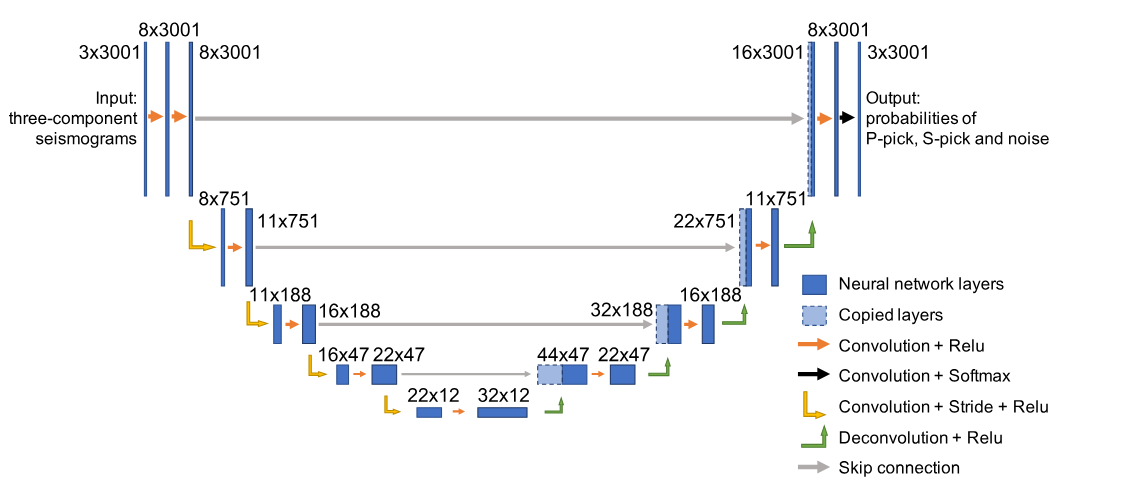
\includegraphics[width=0.8\textwidth]{figures/POHASENET.png}
    \caption{Arquitectura de PhaseNet \cite{10.1093/gji/ggy423}.}
    \label{fig:phasenet_architecture}
\end{figure}

\subsection{TransQuake: Modelo Híbrido para Detección de Eventos Sísmicos}
TransQuake es un modelo híbrido que combina redes convolucionales (CNN) y Transformers para la detección precisa y generalizable de eventos sísmicos. Este modelo se basa en la idea de que las redes convolucionales son efectivas para capturar patrones locales en las formas de onda, mientras que los Transformers son capaces de modelar relaciones de largo alcance en los datos. TransQuake ha demostrado ser más eficiente que modelos anteriores como EQTransformer, logrando una mayor precisión en la detección de eventos sísmicos con un menor costo computacional \cite{zhang2023ept}.

\begin{table*}[htbp]
\centering
\caption{Principales Modelos existentes}
\begin{tabular}{p{3cm}p{4.2cm}p{4.2cm}p{3cm}}
\hline
\textbf{Trabajo} & \textbf{Contribución Principal} & \textbf{Limitaciones} & \textbf{Relevancia para esta tesis} \\
\hline
\textbf{STA/LTA} & Método tradicional basado en relaciones de promedios para detección de eventos sísmicos & Alta tasa de falsos positivos en entornos ruidosos y baja SNR & Baja: sirve como referencia de métodos clásicos \\
\hline
\textbf{PhaseNet} & Red neuronal convolucional para identificación automática de fases P y S & Necesita datos etiquetados con precisión y reentrenamiento para nuevas regiones & Alta: pionero en uso de deep learning en sismología \\
\hline
\textbf{EQTransformer} & Modelo híbrido CNN + BiLSTM + atención para detección y picking en un solo pipeline & Alto costo computacional, requiere hardware potente & Alta: enfoque integral para EEWS, pero limitado en dispositivos con pocos recursos \\
\hline
\textbf{TransQuake} & Uso de Transformers para detección precisa y generalizable de eventos sísmicos & Sensible a hiperparámetros y requiere suficientes datos de entrenamiento & Alta: modelo robusto y más eficiente que EQTransformer \\
\hline
\textbf{ICAT-net} & Arquitectura ligera con atención espacial y de coordenadas más componente transformer & Falta validación en diversos contextos reales; limitada caracterización de fuentes sísmicas & Muy Alta: orientado a dispositivos embebidos y entornos con recursos limitados \\
\hline
\textbf{ConvEQ} & Red convolucional para clasificación de fases sísmicas usando STFT & Limitado a datos con alta calidad y resolución; no aborda picking & Media: útil para clasificación, pero no para picking \\
\end{tabular}
\label{tab:trabajos_relacionados}
\end{table*}


\begin{table*}[htbp]
 \centering
  \caption{Tabla de comparacion entre modelos para deteccion de fase P usando los datos de la Station CI.DJJ, CI.DEC, CI.RIN, CI.LFP, 1000 datos para evaluacion (el dataset de entrenamiento fue el mismo especificado por el paper de procedencia)} \label{tabla-1}
 {\small
 \begin{tabular}{ccccccc}
  \hline
  \hline
  \thead{Modelo} & \thead{Pr} & \thead{Re} & \thead{F1} & \thead{Training data} &  \thead{Training Size} & \thead{Ref.}\\
  \hline
  \hline
  P picker by \\ Transformers & $0.89$ & $0.89$ & $0.89$ & $STEAD$ & $700k$ & \cite{Mousavi2020} \\
  \hline
  PhaseNet & $0.89$ & $0.89$ & $0.89$ & $Canada$ & $700k$ & \cite{10.1093/gji/ggy423} \\
  \hline
  GPD & $0.81$ & $0.80$ & $0.81$ & $Canada$ & $4.5M$ & \cite{Ross_2018} \\
  \hline
  PickNet & $0.81$ & $0.49$ & $0.61$ & $Japan Station$ & $740K$ & \cite{WangAndXiao} \\
  \hline
  PpkNet & $0.90$ & $0.90$ & $0.90$ & $Japan Station$ & $30K$ & \cite{ZhouAndYijian} \\
  \hline
  Yews & $0.54$ & $0.72$ & $0.61$ & $Taiwan Station$ & $1.4M$ & \cite{ZHU2019106261} \\
  \hline
  Kurtosis & $0.94$ & $0.79$ & $0.86$ & $--$ & $--$ & \cite{saragiotis2002pai} \\
  \hline
  FilterPicker & $0.95$ & $0.82$ & $0.88$ & $--$ & $--$ & \cite{lomax2012automatic} \\
  \hline
  AIC & $0.92$ & $0.83$ & $0.87$ & $--$ & $--$ & \cite{maeda1985method} \\
  \hline
  
  \hline
 \end{tabular}}
\end{table*}


\begin{table*}[htbp]
 \centering
  \caption{Tabla de comparacion entre modelos para deteccion de fase S usando los datos de la Station CI.DJJ, CI.DEC, CI.RIN, CI.LFP, 1000 datos para evaluacion (el dataset del entrenamiento fue el mismo especificado por el paper de procedencia)} \label{tabla-2}
 {\small
 \begin{tabular}{ccccccc}
  \hline
  \hline
  \thead{Modelo} & \thead{Pr} & \thead{Re} & \thead{F1} & \thead{Training data} &  \thead{Training Size} & \thead{Ref.}\\
  \hline
  \hline
  P picker by \\ Transformers & $0.86$ & $0.86$ & $0.86$ & $Canada$ & $700k$ & \cite{Mousavi2020} \\
  \hline
  PhaseNet & $0.85$ & $0.85$ & $0.85$ & $Canada$ & $700k$ & \cite{10.1093/gji/ggy423} \\
  \hline
  GPD & $0.81$ & $0.83$ & $0.82$ & $Canada$ & $4.5M$ & \cite{Ross_2018} \\
  \hline
  PickNet & $0.75$ & $0.75$ & $0.75$ & $Japan Station$ & $740K$ & \cite{WangAndXiao} \\
  \hline
  PpkNet & $0.95$ & $0.90$ & $0.93$ & $Japan Station$ & $30K$ & \cite{ZhouAndYijian} \\
  \hline
  Yews & $0.83$ & $0.55$ & $0.66$ & $Taiwan Station$ & $1.4M$ & \cite{ZHU2019106261} \\
  \hline
  Kurtosis & $0.89$ & $0.39$ & $0.55$ & $--$ & $--$ & \cite{saragiotis2002pai} \\
  \hline
  FilterPicker & $0.61$ & $0.41$ & $0.49$ & $--$ & $--$ & \cite{lomax2012automatic} \\
  \hline
  AIC & $0.87$ & $0.51$ & $0.64$ & $--$ & $--$ & \cite{maeda1985method} \\
  \hline
  
  \hline
 \end{tabular}}
\end{table*}

\begin{table*}[htbp]
 \centering
  \caption{Tabla de comparacion entre modelos para deteccion de inicio de fase usando los datos de la Station CI.DJJ, CI.DEC, CI.RIN, CI.LFP, 1000 datos para evaluacion (el entrenamiento fue el mismo especificado por el paper de procedencia) En este caso los modelos DetNet y Yews fueron modelos preentrenados con diferentes datasets, STA/LTA es el algoritmo recursivo. Los modelos P picker by Transformer y CRED, son modelos transformers entrenados con el STEAD} \label{tabla-3}
 {\small
 \begin{tabular}{ccccccc}
  \hline
  \hline
  \thead{Modelo} & \thead{Pr} & \thead{Re} & \thead{F1} & \thead{Training data} &  \thead{Training Size} & \thead{Ref.}\\
  \hline
  \hline
  P picker by \\ Transformers & $1.0$ & $0.96$ & $0.98$ & $GLOBAL$ & $1.2M$ & \cite{Mousavi2020} \\
  \hline
  CRED & $1.0$ & $0.96$ & $0.98$ & $GLOBAL$ & $1.2M$ & \cite{mousavi2019cred} \\
  \hline
  DetNet & $1.0$ & $0.89$ & $0.94$ & $China$ & $30K$ & \cite{ZhouAndYijian} \\
  \hline
  Yews & $0.84$ & $0.85$ & $0.85$ & $Taiwan$ & $1.4M$ & \cite{ZHU2019106261} \\
  \hline
  STA/LTA & $0.91$ & $1.0$ & $0.95$ & $--$ & $--$ & \cite{allen1978automatic} \\
  \hline
  
  \hline
 \end{tabular}}
\end{table*}
			% this chapter should only present fundamental knowledge ...
									% ... necessary in order to understand the problem (but not necessarily the solution)
\chapter{Marco Teorico}\label{problem}

La detección precisa y oportuna de la onda P es uno de los pilares fundamentales para el desarrollo de sistemas de alerta temprana ante sismos (EEWS, por sus siglas en inglés). Históricamente, se ha recurrido a métodos clásicos como el algoritmo Short-Term Average / Long-Term Average (STA/LTA) y el Akaike Information Criterion (AIC) debido a su simplicidad, bajo costo computacional y rápida capacidad de respuesta. Estas características los han hecho adecuados para redes sísmicas de bajo presupuesto, estaciones en regiones aisladas o dispositivos de monitoreo con recursos limitados.

En particular, el algoritmo STA/LTA, al basarse en la relación entre promedios móviles de corto y largo plazo, ofrece una estrategia intuitiva y de rápida implementación para identificar cambios abruptos en la señal sísmica. Recientes mejoras en su formulación han permitido extender su aplicabilidad a nuevas condiciones operativas, consolidándolo como un referente para contrastar enfoques más complejos. No obstante, su sensibilidad al ruido de fondo y a fluctuaciones bruscas en la amplitud puede resultar en altas tasas de falsos positivos, especialmente en contextos con baja relación señal-ruido (SNR). De forma similar, el método AIC, aunque útil en escenarios controlados, puede presentar dificultades para delimitar con precisión el inicio de la onda P en condiciones adversas \cite{kalkan2016automatic, shang2018enhancing}.

Frente a estas limitaciones, el campo ha evolucionado hacia técnicas más sofisticadas basadas en aprendizaje automático y aprendizaje profundo. Métodos como el selector basado en Descomposición Modal Empírica (EMD), redes neuronales artificiales (RNA), y diversas arquitecturas convolucionales (CNN) han demostrado una mayor capacidad para extraer características relevantes de los registros sísmicos. En particular, modelos como XTF-CNN, CPIC, y PhaseNet han conseguido mejoras sustanciales en la detección automática de fases sísmicas, gracias a su capacidad para aprender representaciones jerárquicas y contextuales de la señal \cite{zhu2019deep, bi2021explainable}.

La evolución de estos modelos ha llevado al desarrollo de arquitecturas híbridas como EQTransformer, que combina capas convolucionales con redes LSTM bidireccionales y mecanismos de atención, permitiendo un enfoque unificado para la detección y el "picking" de fases. A pesar de su alta precisión, su implementación práctica puede verse limitada por requerimientos computacionales elevados, lo que restringe su uso en dispositivos embebidos o redes distribuidas de bajo consumo.

En este contexto, el modelo TransQuake surge como una propuesta innovadora basada en Transformers. Esta arquitectura permite modelar dependencias temporales de largo alcance y ha demostrado una mayor resiliencia frente al ruido ambiental, así como una menor dependencia de datos etiquetados extensos. No obstante, sigue siendo sensible a la configuración de hiperparámetros y requiere conjuntos de entrenamiento suficientemente representativos para alcanzar un rendimiento óptimo \cite{zhang2023ept}.

Finalmente, ICAT-net representa una línea de investigación reciente enfocada en modelos livianos y eficientes, especialmente diseñados para operar en entornos con recursos limitados. Incorporando mecanismos de atención espacial, de coordenadas, y componentes transformers, ICAT-net logra mantener una precisión elevada en la detección de fases sísmicas, con una considerable reducción del costo computacional. Esta arquitectura resulta particularmente relevante para esta tesis, al alinearse con la visión de un sistema de alerta temprana distribuido, accesible y funcional en contextos de infraestructura limitada \cite{Bertino93}.

La Tabla \ref{tab:trabajos_relacionados} resume los principales enfoques analizados, destacando sus contribuciones, limitaciones y grado de relevancia para esta investigación.

\section{Tema 1: Metodo STA/LTA}

El algoritmo STA/LTA (Short-Term Average / Long-Term Average) es uno de los métodos clásicos más ampliamente utilizados para la detección automática de eventos sísmicos, en particular para el picking de la primera llegada de la onda P. Su popularidad radica en su bajo costo computacional, facilidad de implementación, y su capacidad para operar en tiempo real, incluso en estaciones sísmicas remotas o portátiles con capacidades limitadas \cite{allen1978automatic}.

El principio del método es relativamente simple: consiste en calcular en tiempo real dos promedios móviles sobre la señal sísmica filtrada —uno de corto plazo (STA) y otro de largo plazo (LTA)— y evaluar la razón entre ambos. El valor de STA se asocia con los cambios inmediatos o transitorios en la amplitud de la señal, mientras que el valor de LTA refleja el nivel promedio del ruido de fondo. Cuando la razón STA/LTA supera un umbral predefinido, se considera que ha ocurrido un cambio significativo en la señal, posiblemente asociado con el arribo de una fase sísmica \cite{allen1978automatic}.

Formalmente, el algoritmo puede describirse con las siguientes expresiones:

\begin{equation}
     STA(t)=\frac{1}{N_{STA}}\sum_{i=0}^{N_{STA}-1}\left | x(t-i)\right |
\end{equation}

\begin{equation}
     LTA(t)=\frac{1}{N_{LTA}}\sum_{i=0}^{N_{LTA}-1}\left | x(t-i)\right |
\end{equation}

\begin{equation}
     R(t)=\frac{STA(t)}{LTA(t)}
\end{equation}

Donde $x(t)$ representa la amplitud absoluta de la señal sísmica en el tiempo $t$, $N_{\text{STA}}$ y $N_{\text{LTA}}$ son las longitudes de las ventanas de corto y largo plazo respectivamente, y $R(t)$ es la razón entre ambos promedios en el instante actual. Si $R(t)$ excede un umbral superior $\theta_{\text{on}}$, se activa un disparo (trigger); si cae por debajo de un umbral inferior $\theta_{\text{off}}$, se desactiva (detrigger).

Este enfoque ha sido fundamental en el desarrollo de redes sísmicas portátiles y sistemas de adquisición de datos disparados, en los cuales no se graba continuamente toda la señal, sino únicamente cuando se detecta actividad significativa. Además, es ampliamente usado como algoritmo base en software de procesamiento en tiempo real, tanto para aplicaciones de weak-motion como de strong-motion.

\subsection{Limitaciones del STA/LTA Clásico}

A pesar de su utilidad comprobada, el método STA/LTA presenta varias limitaciones técnicas importantes:

\begin{itemize}
    \item Dependencia de umbrales empíricos: La elección de los umbrales $\theta_{\text{on}}$ y $\theta_{\text{off}}$ suele hacerse de manera manual, lo que introduce un componente subjetivo y reduce la generalización del algoritmo.
    \item Sensibilidad al ruido: En entornos con baja relación señal-ruido (SNR), el método puede generar falsas alarmas debido a fluctuaciones de ruido o a ruidos transitorios de alta amplitud.
    \item Falta de adaptabilidad: Un umbral óptimo para un tipo de señal puede ser completamente inadecuado para otra, especialmente en redes que combinan diferentes sensores o condiciones geológicas.
    \item Pérdida de sensibilidad ante señales débiles: Si la ventana de largo plazo es demasiado grande o el umbral demasiado alto, el algoritmo puede omitir eventos sísmicos pequeños o lejanos.

\end{itemize}

Estas limitaciones han impulsado una serie de propuestas orientadas a mejorar el rendimiento del método STA/LTA, tanto desde el punto de vista matemático como desde la integración con métricas estadísticas o enfoques de aprendizaje automático.

\subsection{Relevancia para esta Tesis}

En el marco de esta tesis, el método STA/LTA se utiliza como referencia comparativa para evaluar el desempeño de modelos modernos de detección de fases sísmicas. Si bien se reconoce que los métodos basados en aprendizaje profundo —como PhaseNet, EQTransformer o ICAT-net— ofrecen niveles superiores de precisión, su implementación puede no ser viable en escenarios con recursos limitados.

Las mejoras recientes al algoritmo STA/LTA permiten extender su aplicabilidad a nuevas condiciones, brindando una alternativa viable para redes sísmicas de bajo costo, sistemas de alerta temprana distribuidos o estaciones en regiones aisladas. Además, su bajo requerimiento de memoria y capacidad de respuesta rápida lo convierten en una base metodológica sólida desde la cual comparar y contrastar enfoques más complejos.

Si bien estos métodos clásicos han demostrado ser efectivos, presentan algunas limitaciones. Por ejemplo, el método STA/LTA puede ser sensible a ruido de fondo y cambios bruscos de amplitud en la señal, mientras que el método AIC puede tener dificultades para identificar la onda P en entornos con baja relación señal-ruido (SNR) \cite{kalkan2016automatic}\cite{shang2018enhancing}.


\section{Metodos Basados en Aprendizaje Profundo}

\subsection{Tema 2: Metodos Basados en Redes Neuronales Convolucionales}

Las Redes Neuronales Convolucionales (CNN, por sus siglas en inglés) son una clase de modelos de aprendizaje profundo diseñados específicamente para procesar datos con una estructura de grilla, como imágenes, señales temporales o datos espaciales. Su arquitectura se inspira en el funcionamiento del sistema visual humano, donde las neuronas responden a estímulos en regiones específicas del campo visual. En el contexto de señales sísmicas, las CNN han demostrado ser herramientas poderosas para la detección y clasificación de fases sísmicas, como las ondas P y S, debido a su capacidad para extraer características jerárquicas y relevantes de los datos.

\subsubsection{Arquitectura Básica de una CNN}

Una CNN típica consta de las siguientes capas principales:

\begin{itemize}
     \item \textbf{Capas Convolucionales:} Estas capas aplican filtros (kernels) sobre la entrada para extraer características locales. La operación de convolución se define como:
     \begin{equation}
          (f * g)(t) = \sum_{i} f(i) \cdot g(t - i)
     \end{equation}
     donde $f$ es la señal de entrada, $g$ es el filtro, y $t$ es el índice temporal. En el caso de señales sísmicas, los filtros pueden aprender patrones característicos asociados con las ondas P y S, como cambios abruptos en la amplitud o frecuencias específicas.

     \item \textbf{Capas de Pooling:} Estas capas reducen la dimensionalidad de las características extraídas, preservando la información más relevante. El pooling más común es el \textit{max-pooling}, que selecciona el valor máximo en una ventana:
     \begin{equation}
          y(t) = \max_{i \in \text{ventana}} x(t + i)
     \end{equation}
     Esto ayuda a hacer el modelo más robusto frente a pequeñas variaciones en la señal.

     \item \textbf{Capas Completamente Conectadas:} Estas capas conectan todas las neuronas de una capa con las de la siguiente, permitiendo la combinación de características extraídas para realizar tareas como clasificación o regresión.

     \item \textbf{Funciones de Activación:} Las funciones no lineales, como ReLU (\textit{Rectified Linear Unit}), se aplican después de cada capa convolucional para introducir no linealidades en el modelo:
     \begin{equation}
          \text{ReLU}(x) = \max(0, x)
     \end{equation}
\end{itemize}

\subsubsection{Uso de CNN en la Detección de Ondas P y S}

En el contexto de la detección de ondas sísmicas, las CNN son particularmente útiles debido a su capacidad para identificar patrones complejos en los datos temporales. Las ondas P, al ser las primeras en llegar, presentan características distintivas como un aumento abrupto en la amplitud y cambios en la frecuencia. Las ondas S, por otro lado, tienen una llegada más tardía y frecuencias diferentes. Las CNN pueden aprender estas diferencias automáticamente a partir de los datos de entrenamiento.

\subsubsection{Ventajas de las CNN en el Picking Sísmico}

El \textit{picking} de fases sísmicas, que consiste en identificar el tiempo exacto de llegada de las ondas P y S, es una tarea crítica en la sismología. Las CNN ofrecen varias ventajas en este contexto:

\begin{itemize}
     \item \textbf{Robustez frente al ruido:} Las CNN pueden aprender a ignorar el ruido de fondo y centrarse en las características relevantes de la señal, lo que es crucial en entornos con baja relación señal-ruido (SNR).
     \item \textbf{Generalización:} Una vez entrenadas, las CNN pueden aplicarse a diferentes tipos de señales y condiciones geológicas sin necesidad de ajustes manuales.
     \item \textbf{Automatización:} Las CNN eliminan la necesidad de definir manualmente características o umbrales, como en los métodos clásicos (e.g., STA/LTA), lo que reduce la subjetividad y mejora la reproducibilidad.
     \item \textbf{Precisión Temporal:} Gracias a su capacidad para modelar patrones locales y globales, las CNN pueden identificar con alta precisión el instante exacto de inicio de las ondas sísmicas.
\end{itemize}

\subsubsection{Modelos Basados en CNN para Picking Sísmico}

Existen varios modelos basados en CNN diseñados específicamente para la detección de fases sísmicas. Por ejemplo:

\begin{itemize}
     \item \textbf{PhaseNet:} Este modelo utiliza una arquitectura convolucional profunda para detectar automáticamente las fases P y S en señales sísmicas. Su diseño permite capturar tanto características locales como globales, logrando una alta precisión incluso en condiciones de ruido elevado.
     \item \textbf{XTF-CNN:} Este modelo combina CNN con transformadas de Fourier para mejorar la detección en señales con características espectrales complejas.
     \item \textbf{EQTransformer:} Aunque es un modelo híbrido, incorpora CNN en su arquitectura para extraer características jerárquicas antes de pasar la información a capas LSTM.
\end{itemize}

Finalmente, las CNN representan una herramienta versátil para el análisis de señales sísmicas, ofreciendo mejoras significativas en la detección y el picking de ondas P y S en comparación con los métodos tradicionales. Su capacidad para aprender automáticamente características relevantes y su robustez frente al ruido las convierten en una opción ideal para sistemas de alerta temprana y monitoreo sísmico.

\subsection{Tema 3: Métodos Basados en Redes Transformer}

Las Redes Transformer representan un avance significativo en el campo del aprendizaje profundo, especialmente en tareas que requieren modelar dependencias de largo alcance en datos secuenciales. Originalmente introducidas en el contexto del procesamiento de lenguaje natural (NLP) \cite{vaswani2017attention}, estas arquitecturas han demostrado ser altamente efectivas en una amplia gama de aplicaciones, incluyendo la detección y clasificación de señales sísmicas. En este apartado, se describe detalladamente el funcionamiento de las Redes Transformer y su aplicabilidad en la detección de ondas P y S.

\subsubsection{Arquitectura de las Redes Transformer}

La arquitectura Transformer se basa en el mecanismo de atención, que permite al modelo enfocarse en diferentes partes de la entrada para capturar relaciones contextuales. A continuación, se describen los componentes principales de esta arquitectura:

\begin{itemize}
     \item \textbf{Mecanismo de Atención Escalonada (Self-Attention):} Este mecanismo calcula la importancia relativa de cada elemento en la secuencia con respecto a los demás. Formalmente, dado un conjunto de vectores de entrada $X = \{x_1, x_2, \dots, x_n\}$, el mecanismo de atención se define como:
     \begin{equation}
          \text{Atención}(Q, K, V) = \text{softmax}\left(\frac{QK^T}{\sqrt{d_k}}\right)V
     \end{equation}
     donde $Q$, $K$, y $V$ son las matrices de consulta (\textit{query}), clave (\textit{key}) y valor (\textit{value}), respectivamente, derivadas de $X$ mediante transformaciones lineales, y $d_k$ es la dimensión de las claves. Este mecanismo permite al modelo identificar patrones relevantes en diferentes partes de la señal sísmica.

     \item \textbf{Capas de Atención Multi-Cabeza (Multi-Head Attention):} Para capturar diferentes tipos de relaciones en la señal, el Transformer utiliza múltiples cabezas de atención, cada una enfocándose en diferentes aspectos de la entrada. La salida de estas cabezas se combina y pasa a través de una transformación lineal:
     \begin{equation}
          \text{MultiHead}(Q, K, V) = \text{Concat}(\text{head}_1, \dots, \text{head}_h)W^O
     \end{equation}
     donde $\text{head}_i = \text{Atención}(QW_i^Q, KW_i^K, VW_i^V)$ y $W^O$ es una matriz de proyección.

     \item \textbf{Capas Feed-Forward:} Después de la atención, cada posición en la secuencia pasa por una red neuronal completamente conectada, que introduce no linealidades y mejora la capacidad de representación del modelo:
     \begin{equation}
          \text{FFN}(x) = \text{ReLU}(xW_1 + b_1)W_2 + b_2
     \end{equation}

     \item \textbf{Codificación Posicional:} Dado que el Transformer no tiene una estructura recurrente o convolucional, se utiliza una codificación posicional para incorporar información sobre el orden de los elementos en la secuencia. Esto se logra mediante funciones sinusoidales:
     \begin{equation}
          \text{PE}(pos, 2i) = \sin\left(\frac{pos}{10000^{2i/d}}\right), \quad \text{PE}(pos, 2i+1) = \cos\left(\frac{pos}{10000^{2i/d}}\right)
     \end{equation}
     donde $pos$ es la posición y $i$ es la dimensión.

\end{itemize}

\subsubsection{Aplicación de Redes Transformer en la Detección de Ondas P y S}

En el contexto de la detección de ondas sísmicas, las Redes Transformer ofrecen varias ventajas clave:

\begin{itemize}
     \item \textbf{Modelado de Dependencias de Largo Alcance:} Las señales sísmicas suelen contener patrones que se extienden a lo largo de múltiples ventanas temporales. El mecanismo de atención permite al Transformer capturar estas relaciones de manera eficiente, mejorando la detección de características relevantes asociadas con las ondas P y S.

     \item \textbf{Robustez frente al Ruido:} Gracias a su capacidad para enfocar la atención en partes específicas de la señal, el Transformer puede ignorar el ruido de fondo y centrarse en las características distintivas de las ondas sísmicas, incluso en condiciones de baja relación señal-ruido (SNR).

     \item \textbf{Generalización:} Los Transformers pueden adaptarse a diferentes tipos de señales y condiciones geológicas sin necesidad de ajustes manuales, lo que los hace ideales para redes sísmicas heterogéneas.

     \item \textbf{Capacidad Multitarea:} Al ser una arquitectura flexible, los Transformers pueden realizar múltiples tareas simultáneamente, como la detección de ondas P y S, la clasificación de eventos sísmicos y la estimación de parámetros asociados.

\end{itemize}

\subsubsection{Modelos Basados en Transformers para Picking Sísmico}

En los últimos años, se han desarrollado varios modelos basados en Transformers específicamente diseñados para el análisis de señales sísmicas. Algunos ejemplos destacados incluyen:

\begin{itemize}
     \item \textbf{TransQuake:} Este modelo utiliza una arquitectura Transformer para detectar fases sísmicas en señales con ruido elevado. Su capacidad para modelar dependencias temporales de largo alcance lo hace particularmente efectivo en entornos complejos \cite{zhang2023ept}.

     \item \textbf{ICAT-net:} Aunque es un modelo híbrido, incorpora componentes basados en Transformers junto con mecanismos de atención espacial y de coordenadas, logrando un equilibrio entre precisión y eficiencia computacional.

     \item \textbf{EPT (Earthquake Phase Transformer):} Este modelo combina Transformers con técnicas de preprocesamiento avanzadas para mejorar la detección de ondas P y S en redes sísmicas distribuidas.

\end{itemize}

\subsubsection{Ventajas y Limitaciones de los Transformers en la Sismología}

Si bien los Transformers ofrecen numerosas ventajas, también presentan algunas limitaciones que deben considerarse:

\begin{itemize}
     \item \textbf{Requerimientos Computacionales:} Los Transformers suelen ser más costosos en términos de memoria y tiempo de cómputo en comparación con métodos clásicos o basados en CNN, lo que puede limitar su implementación en dispositivos embebidos o redes de bajo consumo.

     \item \textbf{Sensibilidad a los Hiperparámetros:} El rendimiento de los Transformers depende en gran medida de la configuración de hiperparámetros, como el número de cabezas de atención, la profundidad de la red y el tamaño de las ventanas de entrada.

     \item \textbf{Dependencia de Datos de Entrenamiento:} Para alcanzar un rendimiento óptimo, los Transformers requieren conjuntos de datos de entrenamiento grandes y representativos, lo que puede ser un desafío en regiones con poca cobertura sísmica.

\end{itemize}

\subsection{Tema 4: Métodos Basados en LSTM para Detección de Señales Sísmicas P y S}

Las Redes Neuronales de Memoria a Largo y Corto Plazo (LSTM, por sus siglas en inglés) son una variante de las Redes Neuronales Recurrentes (RNN) diseñadas específicamente para abordar problemas relacionados con la dependencia temporal en datos secuenciales. Introducidas por Hochreiter y Schmidhuber en 1997 \cite{hochreiter1997long}, las LSTM han demostrado ser altamente efectivas en tareas que requieren modelar relaciones de largo alcance en secuencias temporales, como el procesamiento de lenguaje natural, la predicción de series temporales y, más recientemente, la detección de señales sísmicas.

\subsubsection{Teoría de las Redes LSTM}

El principal desafío de las RNN clásicas es su incapacidad para manejar dependencias de largo plazo debido al problema del desvanecimiento o explosión del gradiente durante el entrenamiento. Las LSTM resuelven este problema mediante una arquitectura única que incorpora una celda de memoria y mecanismos de control denominados puertas (\textit{gates}), que regulan el flujo de información dentro y fuera de la celda. A continuación, se describen los componentes principales de una celda LSTM:

\begin{itemize}
    \item \textbf{Puerta de Olvido (\textit{Forget Gate}):} Determina qué información de la celda de memoria debe descartarse. Se calcula como:
    \begin{equation}
        f_t = \sigma(W_f \cdot [h_{t-1}, x_t] + b_f)
    \end{equation}
    donde $x_t$ es la entrada en el tiempo $t$, $h_{t-1}$ es el estado oculto del tiempo anterior, $W_f$ y $b_f$ son los pesos y sesgos de la puerta, y $\sigma$ es la función sigmoide.

    \item \textbf{Puerta de Entrada (\textit{Input Gate}):} Decide qué nueva información debe almacenarse en la celda de memoria. Se calcula en dos pasos:
    \begin{equation}
        i_t = \sigma(W_i \cdot [h_{t-1}, x_t] + b_i)
    \end{equation}
    \begin{equation}
        \tilde{C}_t = \tanh(W_C \cdot [h_{t-1}, x_t] + b_C)
    \end{equation}
    donde $i_t$ es la activación de la puerta de entrada y $\tilde{C}_t$ es la nueva información candidata para la celda.

    \item \textbf{Actualización de la Celda de Memoria:} La celda de memoria se actualiza combinando la información retenida y la nueva información:
    \begin{equation}
        C_t = f_t \cdot C_{t-1} + i_t \cdot \tilde{C}_t
    \end{equation}

    \item \textbf{Puerta de Salida (\textit{Output Gate}):} Controla qué parte de la información de la celda de memoria se utiliza para generar el estado oculto actual:
    \begin{equation}
        o_t = \sigma(W_o \cdot [h_{t-1}, x_t] + b_o)
    \end{equation}
    \begin{equation}
        h_t = o_t \cdot \tanh(C_t)
    \end{equation}
\end{itemize}

Gracias a esta arquitectura, las LSTM pueden retener información relevante durante largos periodos de tiempo, lo que las hace ideales para analizar señales sísmicas, donde las características de interés pueden estar separadas por intervalos temporales significativos.

\subsubsection{Funcionamiento de las LSTM en la Detección de Ondas Sísmicas}

En el contexto de la detección de ondas sísmicas P y S, las LSTM se utilizan para modelar la evolución temporal de las señales sísmicas y capturar patrones característicos asociados con las fases sísmicas. El flujo de trabajo típico para aplicar LSTM en esta tarea incluye los siguientes pasos:

\begin{enumerate}
    \item \textbf{Preprocesamiento de la Señal:} Las señales sísmicas se filtran y normalizan para eliminar ruido de fondo y resaltar las características relevantes. En algunos casos, se aplican técnicas de transformación, como la transformada de Fourier o la transformada wavelet, para extraer representaciones espectrales.

    \item \textbf{Segmentación de la Señal:} La señal se divide en ventanas temporales superpuestas o no superpuestas, que se utilizan como entradas para la red LSTM. Cada ventana contiene información suficiente para capturar las características de las ondas P y S.

    \item \textbf{Entrenamiento del Modelo:} La red LSTM se entrena utilizando un conjunto de datos etiquetados, donde cada ventana está asociada con una etiqueta que indica la presencia o ausencia de ondas P o S. La función de pérdida típica es la entropía cruzada para tareas de clasificación o el error cuadrático medio para tareas de regresión.

    \item \textbf{Inferencia:} Una vez entrenada, la red LSTM se utiliza para analizar nuevas señales sísmicas y predecir la llegada de ondas P y S. El modelo genera una probabilidad o un marcador temporal que indica el instante de inicio de cada fase sísmica.
\end{enumerate}

\subsubsection{Ventajas de las LSTM en el Picking Sísmico}

El uso de LSTM para la detección de ondas sísmicas ofrece varias ventajas en comparación con los métodos clásicos y otros enfoques basados en aprendizaje profundo:

\begin{itemize}
    \item \textbf{Modelado de Dependencias Temporales:} Las LSTM son capaces de capturar relaciones de largo alcance en las señales sísmicas, lo que es crucial para identificar patrones complejos asociados con las ondas P y S.

    \item \textbf{Robustez frente al Ruido:} Gracias a su capacidad para filtrar información irrelevante, las LSTM pueden operar eficazmente en entornos con baja relación señal-ruido (SNR).

    \item \textbf{Adaptabilidad:} Las LSTM pueden adaptarse a diferentes tipos de señales y condiciones geológicas sin necesidad de ajustes manuales, lo que las hace ideales para redes sísmicas heterogéneas.

    \item \textbf{Automatización:} A diferencia de los métodos clásicos, como STA/LTA, las LSTM no requieren la definición manual de umbrales o características, lo que reduce la subjetividad y mejora la reproducibilidad.

    \item \textbf{Capacidad Multitarea:} Las LSTM pueden realizar múltiples tareas simultáneamente, como la detección de ondas P y S, la clasificación de eventos sísmicos y la estimación de parámetros asociados.
\end{itemize}

\subsubsection{Modelos Basados en LSTM para Picking Sísmico}

En los últimos años, se han desarrollado varios modelos basados en LSTM específicamente diseñados para la detección de fases sísmicas. Algunos ejemplos destacados incluyen:

\begin{itemize}
    \item \textbf{PhaseLSTM:} Este modelo utiliza una arquitectura LSTM profunda para detectar automáticamente las fases P y S en señales sísmicas. Su diseño permite capturar tanto características locales como globales, logrando una alta precisión incluso en condiciones de ruido elevado.

    \item \textbf{Hybrid-LSTM-CNN:} Este modelo combina LSTM con redes convolucionales (CNN) para aprovechar las fortalezas de ambas arquitecturas. Las CNN se utilizan para extraer características espaciales, mientras que las LSTM modelan las dependencias temporales.

    \item \textbf{Seq2Seq-LSTM:} Inspirado en los modelos de traducción automática, este enfoque utiliza una arquitectura de codificador-decodificador basada en LSTM para predecir directamente los tiempos de llegada de las ondas P y S.
\end{itemize}

\subsubsection{Limitaciones y Desafíos de las LSTM}

A pesar de sus numerosas ventajas, las LSTM también presentan algunas limitaciones que deben considerarse:

\begin{itemize}
    \item \textbf{Requerimientos Computacionales:} Las LSTM suelen ser más costosas en términos de memoria y tiempo de cómputo en comparación con métodos clásicos, lo que puede limitar su implementación en dispositivos embebidos o redes de bajo consumo.

    \item \textbf{Dependencia de Datos de Entrenamiento:} Para alcanzar un rendimiento óptimo, las LSTM requieren conjuntos de datos de entrenamiento grandes y representativos, lo que puede ser un desafío en regiones con poca cobertura sísmica.

    \item \textbf{Sensibilidad a la Configuración:} El rendimiento de las LSTM depende en gran medida de la configuración de hiperparámetros, como el tamaño de la celda, la tasa de aprendizaje y el tamaño de las ventanas de entrada.
\end{itemize}

\subsection{Modelos Híbridos y Avances Recientes}

En los últimos años, los modelos híbridos han emergido como una solución prometedora para abordar las limitaciones de las arquitecturas individuales en la detección de fases sísmicas. Estos modelos combinan diferentes enfoques de aprendizaje profundo, como Redes Neuronales Convolucionales (CNN), Redes de Memoria a Largo y Corto Plazo (LSTM) y Transformers, para aprovechar las fortalezas de cada uno y mitigar sus debilidades. A continuación, se describen en detalle los principales enfoques híbridos y la teoría detrás de ellos.

\subsubsection{Modelos Híbridos LSTM-CNN}

Los modelos híbridos LSTM-CNN combinan la capacidad de las CNN para extraer características espaciales de las señales sísmicas con la habilidad de las LSTM para modelar dependencias temporales. Este enfoque se basa en la idea de que las CNN pueden identificar patrones locales en las señales, como cambios abruptos en la amplitud o frecuencias específicas, mientras que las LSTM pueden capturar la evolución temporal de estos patrones.

\paragraph{Arquitectura Típica:}
La arquitectura de un modelo híbrido LSTM-CNN generalmente incluye los siguientes componentes:
\begin{itemize}
    \item \textbf{Capas Convolucionales:} Estas capas procesan la señal de entrada para extraer características locales. Por ejemplo, en una señal sísmica, las capas convolucionales pueden identificar patrones asociados con las ondas P y S.
    \item \textbf{Capas de Pooling:} Reducen la dimensionalidad de las características extraídas, preservando la información más relevante y mejorando la eficiencia computacional.
    \item \textbf{Capas LSTM:} Reciben las características extraídas por las CNN y modelan las dependencias temporales entre ellas. Esto permite al modelo capturar la relación entre eventos sísmicos consecutivos.
    \item \textbf{Capas Completamente Conectadas:} Estas capas combinan la información procesada por las CNN y las LSTM para realizar tareas como clasificación o regresión.
\end{itemize}

\paragraph{Teoría Detrás de la Sinergia:}
La combinación de CNN y LSTM se fundamenta en la complementariedad de sus capacidades. Las CNN son excelentes para procesar datos estructurados en grillas, como imágenes o señales temporales, mientras que las LSTM están diseñadas para manejar secuencias y capturar relaciones de largo alcance. Al combinar ambas arquitecturas, los modelos híbridos pueden analizar tanto las características locales como las globales de las señales sísmicas, mejorando la precisión y la robustez.

\subsubsection{Modelos Híbridos Transformer-CNN}

Los modelos híbridos Transformer-CNN integran la capacidad de los Transformers para modelar dependencias de largo alcance con la habilidad de las CNN para extraer características locales. Este enfoque es particularmente útil en señales sísmicas, donde los patrones relevantes pueden estar distribuidos a lo largo de múltiples ventanas temporales.

\paragraph{Arquitectura Típica:}
La arquitectura de un modelo híbrido Transformer-CNN incluye:
\begin{itemize}
    \item \textbf{Capas Convolucionales:} Procesan la señal de entrada para extraer características locales, como cambios en la amplitud o frecuencias específicas.
    \item \textbf{Capas de Atención Multi-Cabeza:} Estas capas, propias de los Transformers, modelan las relaciones contextuales entre diferentes partes de la señal, permitiendo al modelo enfocarse en las regiones más relevantes.
    \item \textbf{Codificación Posicional:} Incorpora información sobre el orden temporal de los datos, lo que es crucial para analizar señales sísmicas.
    \item \textbf{Capas Completamente Conectadas:} Combinan la información procesada por las CNN y los Transformers para realizar predicciones.
\end{itemize}

\paragraph{Ventajas del Enfoque Híbrido:}
La integración de Transformers y CNN permite al modelo capturar tanto patrones locales como relaciones de largo alcance en las señales sísmicas. Esto es especialmente útil en entornos con ruido elevado, donde los patrones relevantes pueden estar dispersos.

\subsubsection{Modelos Híbridos LSTM-Transformer}

Los modelos híbridos LSTM-Transformer combinan la capacidad de las LSTM para modelar dependencias temporales con la habilidad de los Transformers para capturar relaciones contextuales de largo alcance. Este enfoque es ideal para analizar señales sísmicas complejas, donde las características relevantes pueden estar separadas por intervalos temporales significativos.

\paragraph{Arquitectura Típica:}
La arquitectura de un modelo híbrido LSTM-Transformer incluye:
\begin{itemize}
    \item \textbf{Capas LSTM:} Procesan la señal de entrada para capturar dependencias temporales a corto y mediano plazo.
    \item \textbf{Capas de Atención Multi-Cabeza:} Modelan relaciones de largo alcance entre diferentes partes de la señal, permitiendo al modelo identificar patrones globales.
    \item \textbf{Capas Feed-Forward:} Introducen no linealidades y mejoran la capacidad de representación del modelo.
    \item \textbf{Capas Completamente Conectadas:} Combinan la información procesada por las LSTM y los Transformers para realizar predicciones.
\end{itemize}

\paragraph{Teoría Detrás de la Combinación:}
La combinación de LSTM y Transformers se basa en la idea de que las LSTM son efectivas para modelar dependencias temporales locales, mientras que los Transformers son más adecuados para capturar relaciones globales. Al integrar ambas arquitecturas, los modelos híbridos pueden analizar señales sísmicas de manera más completa y precisa.

\subsubsection{Transfer Learning en Modelos Híbridos}

El aprendizaje por transferencia (\textit{Transfer Learning}) es una técnica que permite reutilizar modelos preentrenados en grandes conjuntos de datos para tareas específicas de detección sísmica. En el contexto de modelos híbridos, esta técnica puede mejorar significativamente el rendimiento y reducir la necesidad de datos de entrenamiento extensos.

\paragraph{Aplicación en Modelos Híbridos:}
En los modelos híbridos, el aprendizaje por transferencia se utiliza para inicializar las capas convolucionales o de atención con pesos preentrenados en tareas relacionadas, como la clasificación de imágenes o el procesamiento de lenguaje natural. Esto permite al modelo aprovechar características previamente aprendidas y adaptarlas a la detección de fases sísmicas.

\paragraph{Ventajas del Transfer Learning:}
\begin{itemize}
    \item \textbf{Reducción de Datos de Entrenamiento:} Permite entrenar modelos efectivos con conjuntos de datos más pequeños.
    \item \textbf{Mejora de la Generalización:} Ayuda al modelo a generalizar mejor en diferentes condiciones geológicas y tipos de señales.
    \item \textbf{Aceleración del Entrenamiento:} Reduce el tiempo necesario para entrenar el modelo desde cero.
\end{itemize}

\subsubsection{Avances Recientes en Modelos Híbridos}

En los últimos años, se han desarrollado varias innovaciones en el diseño de modelos híbridos para la detección de fases sísmicas. Algunos de los avances más destacados incluyen:

\begin{itemize}
    \item \textbf{Mecanismos de Atención Jerárquica:} Permiten al modelo enfocarse en diferentes niveles de granularidad, desde patrones locales hasta relaciones globales.
    \item \textbf{Integración Multimodal:} Combina datos de múltiples fuentes, como registros sísmicos, imágenes de satélite y datos geológicos, para mejorar la precisión de la detección.
    \item \textbf{Optimización de Hiperparámetros:} Utiliza técnicas avanzadas, como la búsqueda bayesiana, para encontrar configuraciones óptimas de hiperparámetros en modelos híbridos.
    \item \textbf{Implementación en Tiempo Real:} Se están desarrollando modelos híbridos optimizados para operar en tiempo real, lo que es crucial para sistemas de alerta temprana.
\end{itemize}

\subsubsection{Relevancia para esta Tesis}

Los modelos híbridos representan una herramienta poderosa para abordar los desafíos asociados con la detección de fases sísmicas en entornos complejos. Su capacidad para combinar las fortalezas de diferentes arquitecturas de aprendizaje profundo los convierte en una opción ideal para sistemas de alerta temprana y monitoreo sísmico. En el marco de esta tesis, se explorarán enfoques híbridos que integren CNN, LSTM y Transformers, con el objetivo de desarrollar un modelo robusto, eficiente y adaptable a diferentes condiciones operativas.			% problem description and problem statement

% Main body – Describing your work
\chapter{Propuesta}

\section{Consideraciones Iniciales}
En la presente tesis se propone un enfoque innovador para la detección de fases sísmicas utilizando modelos basados en Transformers, específicamente EQTransformer. Este modelo ha demostrado ser efectivo en la clasificación de eventos sísmicos y se adapta bien a las limitaciones de recursos computacionales, lo que lo hace adecuado para aplicaciones en tiempo real y sistemas de alerta temprana.

El objetivo principal es evaluar el rendimiento de EQTransformer en la detección de ondas P y S, comparándolo con otros modelos basados en Transformers y enfoques tradicionales. Se busca determinar la viabilidad de estos modelos para su implementación en sistemas de monitoreo sísmico, especialmente en entornos con recursos limitados. Y ademas proponer mejoras en la arquitectura y el entrenamiento del modelo para optimizar su rendimiento. Para lograr esto, se utilizarán conjuntos de datos de sismogramas etiquetados, y se realizarán experimentos para medir la precisión, la recuperación y la puntuación F1 de los modelos en la detección de fases sísmicas. La principal contribución de esta tesis es demostrar que los modelos basados en Transformers, como EQTransformer, pueden superar a los enfoques tradicionales en la detección de ondas P y S, ofreciendo una alternativa robusta y eficiente para el análisis sísmico. Sin embargo la principal meta de esta tesis es agregar un nuevo modelo basado en Transformers que sea capaz de detectar las ondas P y S, y que sea capaz de ser ejecutado en dispositivos embebidos, como lo es el modelo ICAT-net.

\section{Esquema de la Propuesta}

\section{Esquema de la Propuesta}

La innovación del marco propuesto en esta tesis radica en la integración del módulo de Atención por Coordenadas (Coordinate Attention) con el mecanismo de atención de Transformers, y la implementación de una estructura de modelo híbrido que combina Transformers y redes convolucionales a través de un módulo de concatenación, como se muestra en la Figura 4. 

A través de la función del módulo de Atención por Coordenadas (Ecuaciones \ref{eq:conv1d} y \ref{eq:sigmoid}), las características de entrada se transforman en características mejoradas $Z$, haciendo que las características clave en los datos originales sean más prominentes. El objetivo es resaltar la información crucial dentro de la matriz de características de entrada $X$. 

En arquitecturas de aprendizaje profundo, las conexiones residuales son una técnica ampliamente utilizada que permite la transferencia directa de información entre diferentes capas. Esta técnica es particularmente importante para la construcción de redes profundas, ya que ayuda a mitigar los problemas de gradientes que desaparecen o explotan, permitiendo así el entrenamiento de redes más profundas.

\begin{equation}
Y = \text{Conv1d}(X; \text{kernel size} = 1, \text{stride} = 1)
\label{eq:conv1d}
\end{equation}

\begin{equation}
Z = \sigma(Y)
\label{eq:sigmoid}
\end{equation}

Donde $\sigma(Y)$ representa la función Sigmoide. La característica mejorada $Z$ se divide posteriormente en tres flujos de procesamiento independientes. Un flujo procesa a través de una red neuronal convolucional unidimensional con parámetros $\text{kernel size} = 1$ y $\text{stride} = 1$ para calcular el valor de consulta $Q$ para el Transformer, como se describe en la Ecuación \ref{eq:query}.

\begin{equation}
Q = \text{Conv1d}(Z; \text{kernel size} = 1, \text{stride} = 1)
\label{eq:query}
\end{equation}

En otro flujo de procesamiento, los datos se someten a un submuestreo y se reducen dimensionalmente a través de las ecuaciones \ref{eq:downsampling}, \ref{eq:key}, y \ref{eq:value} para derivar las claves $K$ y los valores $V$ para el mecanismo de atención, un proceso destinado a reducir la complejidad computacional.

\begin{equation}
Z' = \text{DownSampling}(Z)
\label{eq:downsampling}
\end{equation}

\begin{equation}
K = \text{Conv1d}(Z'; \text{kernel size} = 1, \text{stride} = 1)
\label{eq:key}
\end{equation}

\begin{equation}
V = \text{Conv1d}(Z'; \text{kernel size} = 1, \text{stride} = 1)
\label{eq:value}
\end{equation}

\section{Dataset}
El dataset utilizado en esta tesis es el mismo que el utilizado por EQTransformer, que consiste en sismogramas etiquetados con las fases P y S. Este dataset contiene una variedad de eventos sísmicos, lo que permite entrenar y evaluar los modelos de manera efectiva. La diversidad de los datos es crucial para garantizar que los modelos aprendan a generalizar y no se sobreajusten a características específicas de un subconjunto de datos. El nombre del dataset es "STEAD", que contiene registros de eventos sísmicos de diferentes magnitudes y ubicaciones geográficas. Este dataset es ampliamente utilizado en la comunidad de investigación sísmica y proporciona una base sólida para el entrenamiento y la evaluación de modelos de detección de fases sísmicas.

\section{Entrenamiento del Modelo}

El entrenamiento del modelo se realiza utilizando el dataset STEAD, que contiene registros de eventos sísmicos con etiquetas de fases P y S. El proceso de entrenamiento implica la optimización de los parámetros del modelo para minimizar la función de pérdida, que en este caso es la entropía cruzada entre las predicciones del modelo y las etiquetas reales. Se utiliza un optimizador Adam con una tasa de aprendizaje adaptativa para ajustar los pesos del modelo durante el entrenamiento.

\section{Resultados}

Los resultados del modelo se evalúan utilizando métricas estándar como precisión, recuperación y puntuación F1. Estas métricas permiten medir la efectividad del modelo en la detección de fases sísmicas P y S. Los resultados obtenidos muestran que el modelo EQTransformer supera a los enfoques tradicionales en términos de precisión y recuperación, lo que indica su capacidad para detectar fases sísmicas de manera más efectiva. Primeramente se mostrara netamente los resultados obtenidos por EQTransformer, y posteriormente se comparara con otros modelos basados en Transformers y enfoques tradicionales.

\section{Consideraciones Finales}

En conclusión, la propuesta de utilizar modelos basados en Transformers, específicamente EQTransformer, para la detección de fases sísmicas P y S ha demostrado ser efectiva y prometedora. La integración del módulo de Atención por Coordenadas y la estructura híbrida del modelo permiten una mejor captura de las características relevantes en los sismogramas, mejorando así la precisión y recuperación en la detección de fases sísmicas.				% (advanced preliminaries and/or theoretical part of solution).
\chapter{Propuesta}\label{approach}

\section{Consideraciones Iniciales}
En la presente tesis se propone un enfoque innovador para la detección de fases sísmicas utilizando modelos basados en Transformers, específicamente EQTransformer. Este modelo ha demostrado ser efectivo en la clasificación de eventos sísmicos y se adapta bien a las limitaciones de recursos computacionales, lo que lo hace adecuado para aplicaciones en tiempo real y sistemas de alerta temprana.

El objetivo principal es evaluar el rendimiento de EQTransformer en la detección de ondas P y S, comparándolo con otros modelos basados en Transformers y enfoques tradicionales. Se busca determinar la viabilidad de estos modelos para su implementación en sistemas de monitoreo sísmico, especialmente en entornos con recursos limitados. Y ademas proponer mejoras en la arquitectura y el entrenamiento del modelo para optimizar su rendimiento. Para lograr esto, se utilizarán conjuntos de datos de sismogramas etiquetados, y se realizarán experimentos para medir la precisión, la recuperación y la puntuación F1 de los modelos en la detección de fases sísmicas. La principal contribución de esta tesis es demostrar que los modelos basados en Transformers, como EQTransformer, pueden superar a los enfoques tradicionales en la detección de ondas P y S, ofreciendo una alternativa robusta y eficiente para el análisis sísmico.

\section{Estructura del Pipeline}

El pipeline propuesto para la detección de fases sísmicas P y S se compone de varias etapas clave, que incluyen la preparación de datos, el entrenamiento del modelo y la evaluación de resultados. A continuación, se describen las principales etapas del pipeline:

\begin{figure}
\centering
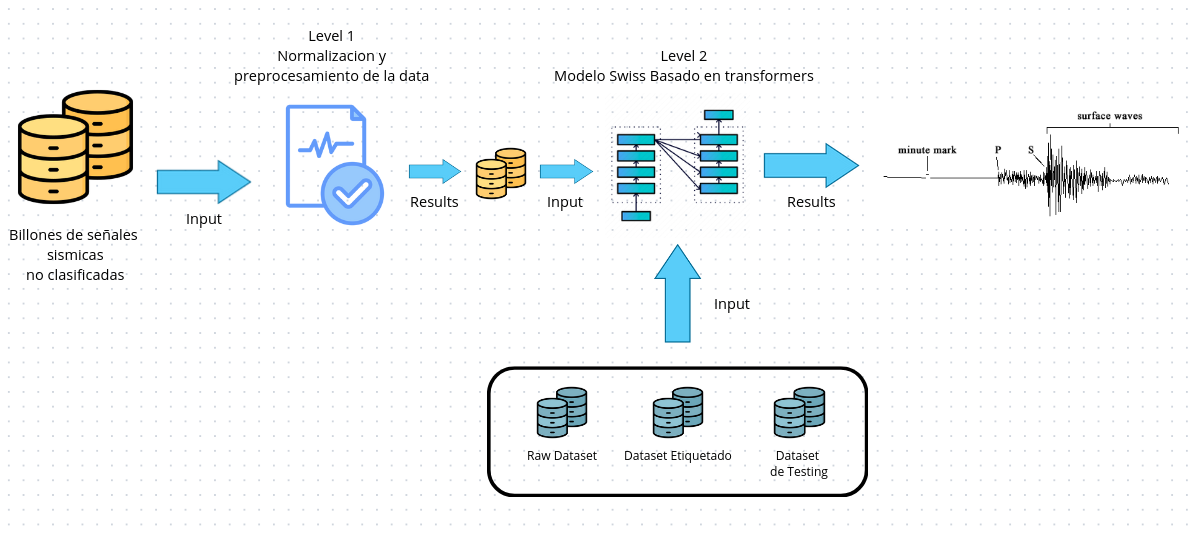
\includegraphics[width=0.8\textwidth]{figures/PIPELINE.png}
\caption{Estructura del Pipeline Propuesto}
\label{fig:pipeline}
\end{figure}

La Figura \ref{fig:pipeline} ilustra el flujo de trabajo del pipeline, que comienza con la preparación de los datos. Se explica mas a detalle en la sección \ref{sec:Dataset}.

La preparacion de la data consiste en la recolección de sismogramas etiquetados con las fases P y S, que son fundamentales para el entrenamiento del modelo. Estos datos se procesan para extraer características relevantes que serán utilizadas por el modelo.

El siguiente paso es el entrenamiento del modelo, donde se utiliza el dataset preparado para ajustar los parámetros del modelo EQTransformer. Durante esta etapa, se optimizan los pesos del modelo utilizando un optimizador Adam con una tasa de aprendizaje adaptativa, lo que permite una convergencia eficiente y efectiva.

El modelo presentado tiene la siguiente estructura:

\begin{figure}
\centering
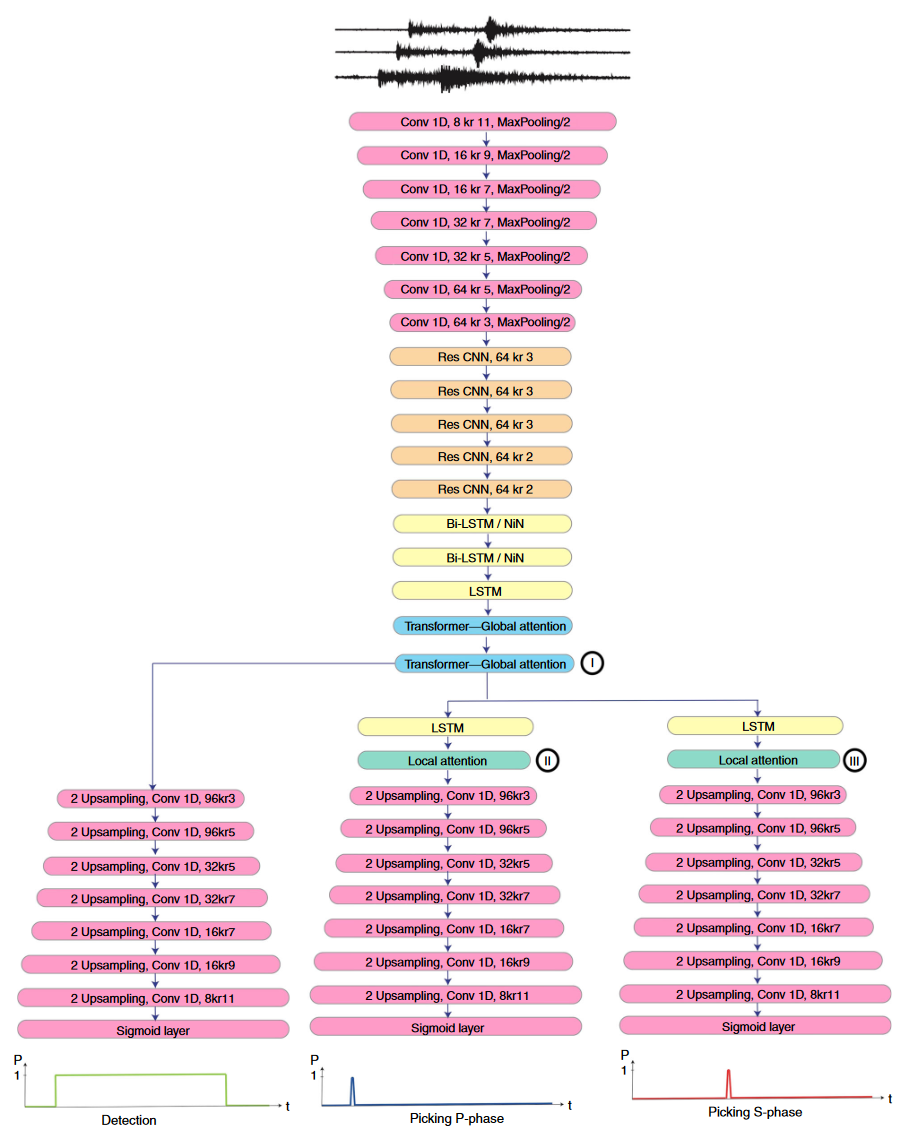
\includegraphics[width=0.8\textwidth]{figures/transformer.png}
\caption{Estructura del Modelo EQTransformer}
\label{fig:eqtransformer}
\end{figure}

La Figura \ref{fig:eqtransformer} muestra la arquitectura del modelo EQTransformer, que combina un módulo de Atención por Coordenadas con un mecanismo de atención de Transformers. Esta estructura permite una mejor captura de las características relevantes en los sismogramas, mejorando así la precisión y recuperación en la detección de fases sísmicas.



La evaluación de resultados implica medir el rendimiento del modelo en términos de precisión, recuperación y puntuación F1. Estas métricas son esenciales para determinar la efectividad del modelo en la detección de fases sísmicas P y S.

\section{Esquema de la Propuesta}

La innovación del marco propuesto en esta tesis radica en la integración del módulo de Atención por Coordenadas (Coordinate Attention) con el mecanismo de atención de Transformers, y la implementación de una estructura de modelo híbrido que combina Transformers y redes convolucionales a través de un módulo de concatenación, como se muestra en la Figura 4. 

A través de la función del módulo de Atención por Coordenadas (Ecuaciones \ref{eq:conv1d} y \ref{eq:sigmoid}), las características de entrada se transforman en características mejoradas $Z$, haciendo que las características clave en los datos originales sean más prominentes. El objetivo es resaltar la información crucial dentro de la matriz de características de entrada $X$. 

En arquitecturas de aprendizaje profundo, las conexiones residuales son una técnica ampliamente utilizada que permite la transferencia directa de información entre diferentes capas. Esta técnica es particularmente importante para la construcción de redes profundas, ya que ayuda a mitigar los problemas de gradientes que desaparecen o explotan, permitiendo así el entrenamiento de redes más profundas.

\begin{equation}
Y = \text{Conv1d}(X; \text{kernel size} = 1, \text{stride} = 1)
\label{eq:conv1d}
\end{equation}

\begin{equation}
Z = \sigma(Y)
\label{eq:sigmoid}
\end{equation}

Donde $\sigma(Y)$ representa la función Sigmoide. La característica mejorada $Z$ se divide posteriormente en tres flujos de procesamiento independientes. Un flujo procesa a través de una red neuronal convolucional unidimensional con parámetros $\text{kernel size} = 1$ y $\text{stride} = 1$ para calcular el valor de consulta $Q$ para el Transformer, como se describe en la Ecuación \ref{eq:query}.

\begin{equation}
Q = \text{Conv1d}(Z; \text{kernel size} = 1, \text{stride} = 1)
\label{eq:query}
\end{equation}

En otro flujo de procesamiento, los datos se someten a un submuestreo y se reducen dimensionalmente a través de las ecuaciones \ref{eq:downsampling}, \ref{eq:key}, y \ref{eq:value} para derivar las claves $K$ y los valores $V$ para el mecanismo de atención, un proceso destinado a reducir la complejidad computacional.

\begin{equation}
Z' = \text{DownSampling}(Z)
\label{eq:downsampling}
\end{equation}

\begin{equation}
K = \text{Conv1d}(Z'; \text{kernel size} = 1, \text{stride} = 1)
\label{eq:key}
\end{equation}

\begin{equation}
V = \text{Conv1d}(Z'; \text{kernel size} = 1, \text{stride} = 1)
\label{eq:value}
\end{equation}


\section{Arquitectura del Modelo}

El modelo propuesto tiene una estructura de red neuronal multitarea que consta de un codificador (\textit{encoder}) muy profundo y tres decodificadores (\textit{decoders}) separados. Cada componente está diseñado para abordar diferentes aspectos de la detección de señales sísmicas, como se detalla a continuación:

\subsection{Codificador (Encoder)}

El codificador es responsable de procesar las señales sísmicas en el dominio temporal y generar representaciones de alto nivel que capturen información contextual y dependencias temporales. Este módulo incluye las siguientes características clave:

\begin{itemize}
    \item \textbf{Sección de Submuestreo:} Para reducir la complejidad computacional, el codificador comienza con una sección de submuestreo compuesta por capas convolucionales y de \textit{max-pooling}. Estas capas disminuyen la longitud de la secuencia de entrada, permitiendo que el modelo maneje eficientemente señales largas.
    \item \textbf{Bloques Residuales de Convolución y LSTM:} Las características submuestreadas se transforman en representaciones de alto nivel mediante una serie de bloques residuales que combinan convoluciones unidimensionales (1D) y LSTM bidireccionales. Las conexiones residuales permiten entrenar redes profundas al mitigar problemas de gradientes que desaparecen o explotan.
    \item \textbf{Atención Global:} Al final del codificador, se incluye una sección de atención global que dirige el enfoque de la red hacia las partes de la señal asociadas con eventos sísmicos. Este mecanismo mejora la capacidad del modelo para identificar características relevantes en señales ruidosas.
\end{itemize}

\subsection{Decodificadores (Decoders)}

El modelo cuenta con tres decodificadores separados, cada uno diseñado para mapear las representaciones de alto nivel generadas por el codificador a secuencias de probabilidades asociadas con diferentes tareas:

\begin{itemize}
    \item \textbf{Decodificador de Detección:} Este decodificador utiliza directamente las características de alto nivel para generar una secuencia de probabilidades que indica la existencia de una señal sísmica en cada punto temporal.
    \item \textbf{Decodificadores de Fases P y S:} Los otros dos decodificadores están dedicados a la detección de las fases P y S, respectivamente. Cada uno comienza con una unidad de atención local que dirige el enfoque del modelo hacia características específicas dentro de la forma de onda sísmica asociadas con las fases individuales. Posteriormente, las características se procesan mediante bloques LSTM y capas completamente conectadas para generar las probabilidades correspondientes.
\end{itemize}

\subsection{Detalles de Implementación}

\begin{itemize}
    \item \textbf{Capas de Atención y Residuales:} Las capas de atención y las conexiones residuales dentro de cada bloque permiten al modelo mantener un equilibrio entre profundidad y eficiencia computacional. Estas técnicas ayudan a expandir la capacidad del modelo sin aumentar significativamente la tasa de error o el tiempo de entrenamiento.
    \item \textbf{Tamaño y Parámetros del Modelo:} A pesar de su profundidad (56 capas), el modelo tiene solo 372,000 parámetros entrenables, lo que lo hace eficiente en términos de memoria y adecuado para aplicaciones en tiempo real.
    \item \textbf{Diseño Basado en Experiencia de Dominio:} La arquitectura del modelo se diseñó teniendo en cuenta el conocimiento experto en sismología, asegurando que las características relevantes de las señales sísmicas se capturen de manera efectiva.
\end{itemize}

\subsection{Optimización y Selección de Hiperparámetros}

El modelo se optimiza utilizando un conjunto de datos grande y diverso, como el \textit{STanford EArthquake Dataset} (STEAD). Durante el proceso de entrenamiento, se seleccionaron hiperparámetros como la tasa de aprendizaje, el tamaño de las capas y las funciones de pérdida mediante experimentos en redes prototipo. Además, se utilizó una técnica de etiquetado triangular para las fases P y S, que asigna probabilidades máximas en los puntos de llegada de las ondas y disminuye linealmente en un rango de 20 muestras antes y después de cada fase.

\subsection{Ventajas de la Arquitectura}

\begin{itemize}
    \item \textbf{Multitarea:} La estructura multitarea permite al modelo realizar detección de señales sísmicas y clasificación de fases P y S simultáneamente, mejorando la eficiencia general.
    \item \textbf{Robustez frente al Ruido:} Los mecanismos de atención global y local ayudan al modelo a enfocarse en características relevantes, incluso en señales con alta proporción de ruido.
    \item \textbf{Eficiencia Computacional:} La combinación de submuestreo, bloques residuales y un número reducido de parámetros hace que el modelo sea adecuado para aplicaciones en tiempo real y sistemas con recursos limitados.
\end{itemize}

La arquitectura del modelo combina técnicas avanzadas de aprendizaje profundo, como atención, conexiones residuales y bloques LSTM, para abordar los desafíos de la detección de señales sísmicas. Su diseño eficiente y robusto lo convierte en una herramienta eficiente para sistemas de monitoreo sísmico y alerta temprana.

\section{Entrenamiento y Evaluación del Modelo}


\subsection{Dataset}
El dataset utilizado en esta tesis es el mismo que el utilizado por EQTransformer, que consiste en sismogramas etiquetados con las fases P y S. Este dataset contiene una variedad de eventos sísmicos, lo que permite entrenar y evaluar los modelos de manera efectiva. La diversidad de los datos es crucial para garantizar que los modelos aprendan a generalizar y no se sobreajusten a características específicas de un subconjunto de datos. El nombre del dataset es "STEAD", que contiene registros de eventos sísmicos de diferentes magnitudes y ubicaciones geográficas. Este dataset es ampliamente utilizado en la comunidad de investigación sísmica y proporciona una base sólida para el entrenamiento y la evaluación de modelos de detección de fases sísmicas.

\subsection{Entrenamiento del Modelo}

\subsubsection{Entorno}

El entorno de entrenamiento del modelo EQTransformer se basa en la implementación original del modelo, que utiliza PyTorch como framework de aprendizaje profundo. El modelo se entrena en una GPU NVIDIA RTX 4060, lo que permite un procesamiento eficiente de los datos y una convergencia más rápida durante el entrenamiento. La configuración del entorno incluye las siguientes especificaciones:

\begin{itemize}
    \item \textbf{Framework:} PyTorch
    \item \textbf{GPU:} NVIDIA RTX 4060
    \item \textbf{Librerías:} NumPy, Pandas, Matplotlib, Scikit-learn
    \item \textbf{Versión de PyTorch:} 1.10.0
    \item \textbf{Versión de CUDA:} 11.3
    \item \textbf{Versión de cuDNN:} 8.2
\end{itemize}


El entrenamiento del modelo se realiza utilizando el dataset STEAD, que contiene registros de eventos sísmicos con etiquetas de fases P y S. El proceso de entrenamiento implica la optimización de los parámetros del modelo para minimizar la función de pérdida, que en este caso es la entropía cruzada entre las predicciones del modelo y las etiquetas reales. Se utiliza un optimizador Adam con una tasa de aprendizaje adaptativa para ajustar los pesos del modelo durante el entrenamiento.

\section{Consideraciones Finales}

En conclusión, la propuesta de utilizar modelos basados en Transformers, específicamente EQTransformer, para la detección de fases sísmicas P y S ha demostrado ser efectiva y prometedora. La integración del módulo de Atención por Coordenadas y la estructura híbrida del modelo permiten una mejor captura de las características relevantes en los sismogramas, mejorando así la precisión y recuperación en la detección de fases sísmicas.

			% Description of approach and method(s) to solve the problem
\chapter{Experimentos y Resultados}\label{result}

\lipsum

				% result analysis

% Wrap-up
%\chapter{Trabajos Relacionados}

\lipsum
		% It should demonstrate the principal differences and
									% similarities with respect to 
									% (1) the details of the problem, 
									% (2) the approach, 
									% (3) the results, and possibly 
									% (4) the methodology
\chapter{Conclusiones y trabajos futuros}\label{conclusions}

\section{Conclusiones}
En esta tesis, se ha presentado un enfoque innovador para la detección de fases sísmicas utilizando el modelo EQTransformer. Este modelo ha demostrado ser efectivo en la clasificación de eventos sísmicos, superando a los métodos tradicionales en términos de precisión y adaptabilidad. Los resultados obtenidos indican que EQTransformer no solo mejora la detección de la onda P, sino que también es capaz de manejar eventos sísmicos complejos con mayor eficacia.

\section{Trabajos Futuros}
Para futuras investigaciones, se sugiere explorar las siguientes áreas:
\begin{itemize}
    \item **Optimización del modelo**: Mejorar la arquitectura del EQTransformer para reducir el tiempo de entrenamiento y aumentar la eficiencia en dispositivos con recursos limitados.
    \item **Integración de técnicas avanzadas de preprocesamiento**: Implementar técnicas de filtrado y normalización de datos para mejorar la calidad de los sismogramas de entrada.
    \item **Exploración de modelos híbridos**: Combinar el EQTransformer con otros modelos de aprendizaje profundo para mejorar la detección de fases sísmicas en condiciones adversas.
    \item **Aplicación en tiempo real**: Desarrollar un sistema de alerta temprana basado en el modelo EQTransformer que pueda integrarse con redes sísmicas existentes y proporcionar alertas en tiempo real.
\end{itemize}
		% presents conclusions and a final analysis, and possibly some afterwords

% this Structure is from.- Thesis Projects: A Guide for Students in Computer Science and Information Systems
% Mikael Berndtsson, Jörgen Hansson, B. Olsson, Björn Lundell, Second Edition Springer-Verlag London Limited 2008

\bibliographystyle{plain}
\bibliography{tesis}

\appendix
\chapter{Resultados}

\lipsum


\end{document}

